\chapter{Úvod}
Wi-Fi sítě můžeme v dnešní době nalézt opravdu téměř kdekoliv -- ve firmách, kavárnách, ale především i v domácnostech. Z důvodu tak hojného využívání je nutné tyto sítě dobře zabezpečit, aby nemohlo docházet například k odposlechu dat. Od roku 1997 byla vydána rada nových bezpečnostních standardů, i přes to však v dnešní době obsahuje zabezpečení Wi-Fi sítí spoustu chyb a nedostatků. Tato bakalářská práce se zabývá problémy v jednotlivých způsobech zabezpečení Wi-Fi sítí a jejich následnému využití k prolomení zabezpečení. Obsahem práce je i přehled nejpoužívanějších nástrojů pro útoky na Wi-Fi sítě -- včetně ukázek jejich použití, následného testování a vyhodnocení. V další části se práce zabývá návrhem a implementací nástroje pro odposlech komunikace mezi klientem a přístupovým bodem -- tento nástroj je vytvořen jak pro samostatná zařízení, tak i pro sondu vyvíjenou na FIT VUT. 

Hlavní motivací práce je poukázat na problémy zabezpečení Wi-Fi sítí a na snadné prolomení špatně zabezpečených sítí. Kapitola \ref{zabezpeceni} pojednává o struktuře Wi-Fi sítí, především pak o přístupových bodech. Dále obsahuje nejznámější metody zabezpečení Wi-Fi sítí a~přehled jejich nedostatků. Následuje kapitola \ref{prolomeni}, která se zabývá existujícími možnostmi pro prolomení zabezpečení Wi-Fi sítí. Zkoumá známé útoky a vysvětluje jejich princip. Také se zabývá detekovatelností jednotlivých útoků. Konec kapitoly poukazuje na bezpečností chyby v několika zařízeních, které jsou v České republice hojně využívány. V rámci kapitoly \ref{nastroje} je uveden seznam nejpoužívanějších nástrojů pro útoky na Wi-Fi sítě. Kapitola obsahuje ukázky použití těchto nástrojů a výčet jejich možností. Následně obsahuje přehled testování nástrojů pro prolamování protokolů WEP a WPA/WPA2. Kapitola je zakončena vyhodnocením a zvolením nejlepšího nástroje. Kapitola \ref{navrh} se zabývá návrhem nástroje pro odposlech dat mezi klientem a přístupovým bodem, popis implementace tohoto nástroje je uveden v kapitole \ref{implementace}.

\chapter{Wi-Fi sítě a jejich zabezpečení} 
\label{zabezpeceni}

Tato kapitola pojednává o struktuře Wi-Fi sítí a o možnostech jejich zabezpečení. 

\section{Struktura Wi-Fi sítí}

Wi-Fi je označení pro bezdrátové sítě využívajících standardů IEEE 802.11, které jsou definovány Institutem pro elektrotechnické a elektronické inženýrství (IEEE) \cite{beaver2015hacking}. Jedná se o infrastrukturní či Ad-hoc sítě. Používány jsou jak pro domácí, tak i pro firemní sítě.

U Ad-hoc síti jde o spojení dvou klientů v rovnocenné pozici, tzv. peer-to-peer připojení, komunikujících spolu za pomocí SSID. Klienti musí být v přímém rádiovém dosahu~\cite{ad-hocSecuring}. Ad-hoc sítě neobsahují žádný přístupový bod ani centrální prvek řídící komunikaci. Infrastrukturní sítě obsahují jeden nebo více přístupových bodů vysílajících svoje SSID, tzv.~Access~point~(AP). SSID není unikátní, několik přístupových bodů tedy může mít stejné SSID. Přístupové body koordinují síťový provoz mezi jednotlivými uzly, často spojují uzly se samotnou sítí a zastávají tak role mostů či routerů.

Klienti se do Wi-Fi sítě připojují přes přístupový bod. Komunikace mezi klienty v síti následně neprobíhá přímo, ale právě za pomoci přístupových bodů -- klienti tedy nemusí být ve vzájemném dosahu. 
\begin{itemize}
  \item{Přístupové body pravidelně vysílají signál, aby se klient o síti dozvěděl. Pro připojení k přístupovému bodu je nutné BSSID i SSID a přístupové body si mohou určovat, který klient se do sítě smí připojit \cite{burns2007security}.}
  \item{Každý přístupový bod představuje síť označenou jako základní balíček služeb neboli BSS. BSS lze identifikovat za pomocí BSSID, což je obvykle MAC adresa přístupového bodu. Každý přístupový bod je také součástí rozšířené sady služeb (ESS). ESS je identifikována za pomocí ESSID či SSID, které většinou tvoří textový řetězec.}
  \item{Úkolem přístupových bodů je také zajistit přenos mezi jednotlivými klienty.}
\end{itemize}

Bezdrátové sítě jsou v dnešní době hojně využívány. Oproti kabelovému spojení nabízejí mnohdy velké usnadnění přístupu do sítě. Jelikož je však veškerá komunikace přenášena vzduchem, v případě špatného či žádného zabezpečení může útočník provoz odposlouchávat, nebo jej nějakým způsobem narušovat a měnit.

\subsection{Přehled standardů}
V roce 1997 vyšel první standard IEEE 802.11. Od vydání prvního standardu utekla již dlouhá doba a tak bylo nutné postupně vydávat nové standardy, které odpovídají požadavkům a nárokům nejnovějších technologií. Tabulka \ref{table:standardy} zobrazuje přehled nejznámějších a nejpoužívanějších standardů IEEE 802.11.

\begin{table}[htb]
\centering
\begin{tabular}{|c|c|c|c|c|}
\hline
\textbf{IEEE Standard} & \textbf{Rok} & \textbf{Frekvence} & \textbf{Maximální propustnost} &\textbf{Dosah} \\ \hline
802.11                 & 1997         & 2,4 GHz            & 2 Mbit/s                       & $\sim$80 m     \\ \hline
802.11a                & 1999         & 5 GHz              & 54 Mbit/s                      & $\sim$120 m     \\ \hline
802.11b                & 1999         & 2,4 GHz              & 11 Mbit/s                      & $\sim$135 m     \\ \hline
802.11g                & 2003         & 2,4 GHz              & 54 Mbit/s                      & $\sim$135 m     \\ \hline
802.11n                & 2009         & 2,4/5 GHz              & 600 Mbit/s                      & $\sim$250 m     \\ \hline
802.11ac            & 2014         & 5 GHz              & 1 Gbit/s                      & $\sim$305 m     \\ \hline
802.11af            & 2014         & 54-790 MHz              & 26,7 Mbit/s                      & $\sim$1000 m     \\ \hline
802.11ad            & 2016         & 60 GHz              & 6,76 Gbit/s                      & $\sim$10 m     \\ \hline
802.11ah            & 2016         & 900 MHz              & 40 Mbit/s                      & $\sim$1000 m     \\ \hline
\end{tabular}
\caption{Přehled nejpoužívanějších standardů IEEE 802.11.}
\label{table:standardy}
\end{table}

\subsection{Rámce bezdrátové sítě}
Sítě dle standardu IEEE 802.11 používají datové, řídící a kontrolní rámce. Datové rámce přenáší samotná skutečná data. Řídící rámce zajišťují propojení stanic a přenos konfigurace sítě. Kontrolní rámce zajišťují usnadnění při výměně datových rámců. Obrázek \ref{img:komunikace} zobrazuje sled řídících rámců při vstupu klienta do sítě. Řídící rámce mohou mnohdy obsahovat důležité informace:
\begin{itemize}
  \item{\textbf{Beacon frame} -- přenáší nejpodstatnější informace o síti. Přístupové body je vysílají pravidelně 10x až 100x za sekundu a vyzývají tak stanice v dosahu k připojení do sítě. Beacon frame obsahuje zejména:
    \begin{itemize}
      \item{\textbf{SSID} -- pokud není skryto,}
      \item{\textbf{časovou známku} -- pro synchronizaci lokálního času,}
      \item{\textbf{Beacon interval} -- interval mezi jednotlivými Beacon rámci,}
      \item{\textbf{informace o způsobilosti} -- 16 bitů obsahující informace o způsobilosti sítě.}
    \end{itemize}
  }
  \item{\textbf{Probe request} -- zasílá ho klient přístupovému bodu jako žádost o připojení do sítě. Obsahuje informace o síti podobné obsahu Beacon rámce.}
  \item{\textbf{Probe response} -- zasílá jej přístupový bod jako odpověď klientovi. Obsahuje informace o síti a její způsobilosti. Na každý probe request připadá jeden probe response.}
  \item{\textbf{Autentizační požadavek} -- klient zasílá autentizační požadavek přístupovému bodu v moment, kdy se chce do sítě připojit. Existuje několik druhů autentizace určených konfigurací sítě. Využívá se otevřená autentizace nebo autentizace se sdíleným klíčem.}
  \item{\textbf{Autentizační odpověď} -- odpověď na autentizační požadavek. Obsahuje informace o stavu nebo výzvu spojenou se sdíleným klíčem. Na každý autentizační požadavek připadá jedna autentizační odpověď.}
  \item{\textbf{Asociační žádost} -- využívají ji klienti v případě skrytého SSID. Musí obsahovat SSID a obsahuje stejné informace jako probe request.}
  \item{\textbf{Asociační odpověď} -- odpověď klientovi na asociační žádost. Obsahuje informace o síti a informace o úspěchu či neúspěchu asociace. Na každý asociační požadavek připadá jedna asociační odpověď.}
  \item{\textbf{Deautentizační rámce} -- jsou odesílány jako upozornění na neúspěšnou autentizaci či asociaci. Dochází k vynucení odpojení klienta od sítě.}
\end{itemize}

\begin{figure}[htbp]
  \centering
  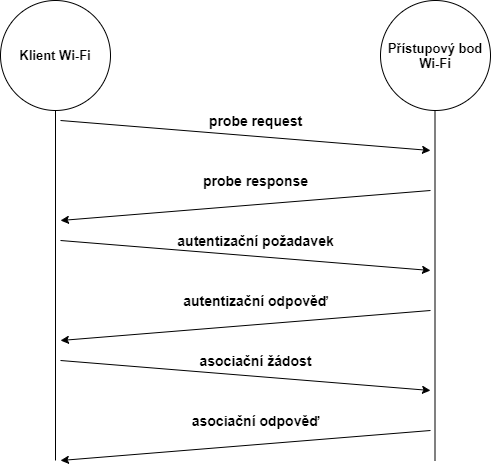
\includegraphics[width=10cm]{obrazky-figures/komunikace.png}
  \caption{Znázornění komunikace mezi klientem a přístupovým bodem při připojování klienta do sítě.}
  \label{img:komunikace}
\end{figure}

\section{Problémy přístupových bodů}
Prakticky každý přístupový bod má svoje slabé místo -- ať už kvůli zjištěným mezerám v samotných standardech či kvůli jejich špatné konfiguraci. Wardriving (vyhledávání Wi-Fi sítí osobou jedoucí ve vozidle za pomocí přenosného zařízení) v největších městech po celém světě ukázal, že drtivá většina přístupových bodů je špatně nakonfigurována či využívá základní konfigurace. Mezi hlavní problémy přístupových bodů patří:
\begin{itemize}
  \item{\textbf{Konfigurace} -- přístupové body obsahují často v základní konfiguraci slabá hesla obsahující 5-12 tisknutelných ASCII znaků. V případě použití zastaralého WEP šifrování je pro útočníka opravdu snadné takové heslo prolomit. Například u routerů od společnosti UPC bylo v roce 2016 odhaleno slabé generování výchozích hesel. Na základě výchozího SSID routeru dodaného od UPC bylo tak možné jednoduše vygenerovat jeho výchozí heslo \cite{UPCPassword}.}
  \item{\textbf{Rogue AP} -- jedná se o přístupové body, které byly nainstalovány do zabezpečené sítě bez autorizace administrátora dané sítě. Mnohdy takový přístupový bod nainstaluje například zaměstnanec společnosti, za účelem zlepšení signálu sítě ve své kanceláři. Útočník takové přístupové body dokáže lehce odhalit a využít k napadení sítě \cite{beyah2004rogue}.}
  \item{\textbf{Trojan AP} -- jde o podobný případ jako u Rogue AP. V tomto případě však přístupový bod instaluje sám útočník a to nejčastěji do míst, kde má skutečný přístupový bod nedostačující signál. Útočník tak může nalákat uživatele k připojení na jeho podvržený přístupový bod, jelikož bude nabízet lepší připojení.}
  \item{\textbf{Výrobci koncových zařízení} -- často se chyb v bezpečnosti koncových zařízení mohou dopustit samotní výrobci, kteří mohou nevědomky vytvořit v samotném zařízení bezpečnostní chybu.}
\end{itemize}

\section{Možná bezpečnostní opatření}
Moderní síťové prvky přináší velkou škálu možností zabezpečení bezdrátových sítí před zneužitím. V dnešní době se používají zejména protokoly WEP, WPA, WPA2 a nově i~WPA3. Existují však i další nástroje a možnosti, které mohou zabránit útočníkovi v narušení sítě.

\subsection{Skrytí SSID}
Jedná se o nejjednodušší, zároveň však nejméně efektivní metodu zabezpečení bezdrátové sítě. Každá síť využívající protokolu IEEE 802.11 vysílá Beacon rámce s informací o dané síti \cite{IdentifyingChannel}. V případě, kdy dojde ke skrytí SSID, pak zařízení posílá SSID o nulové délce, nebo SSID vyplněné nulovými bajty. Skrývání SSID tedy není součástí standardu 802.11, ve skutečnosti jde proti němu \cite{IEEE2016}.

Pokud je SSID skryto, uživatel se může do sítě připojit zasláním takzvaného probe requestu přístupovému bodu. Součástí probe requestu je i SSID přístupového bodu. Následně od přístupového bodu obdrží probe response. To značně snižuje uživatelskou přívětivost sítě, jelikož pro připojení do takové sítě musí uživatel znát SSID a sám se k ní připojit, síť totiž nebude uvedena v seznamu dostupných sítí.

Nalezení skrytého SSID je poměrně snadné i pro běžného uživatele. Stačí k tomu 802.11 adaptér s podporou pro monitorující mód a běžně dostupný software. Za pomocí těchto nástrojů může uživatel zachytit rámce, aniž by byl do sítě připojen. Tyto rámce může poté zanalyzovat. V případě skrytého SSID sice u Beacon paketů SSID chybí, dá se však nalézt například v probe response.

Tato metoda tedy snižuje uživatelskou přívětivost a navíc neposkytuje téměř žádné zvýšení bezpečnosti sítě -- skryté SSID může naopak zvýšit zájem potencionálního útočníka.

\subsection{Filtrování MAC adres}
Další z jednoduchých a opět ne zrovna efektivních metod. Přístupové body obsahují filtr MAC adres zařízení, kterým umožňují přístup do sítě. Útočníkovi však stačí odposlouchávat pakety a získat z nich MAC adresu povoleného zařízení. Následně tuto MAC adresu naklonovat na svoji síťovou kartu a vydávat se tak v síti za dané zařízení. V moment, kdy útočník získá MAC adresu povoleného zařízení, pak vynutí odpojení tohoto zařízení od sítě a následně se do ní sám připojí. 

\subsection{WEP}
Provoz na bezdrátové síti je možné snadno odposlouchávat, jelikož samotný přenos většinou probíhá za pomocí elektromagnetických vln. Z tohoto důvodu je nutné veškerou komunikaci šifrovat tak, aby ji mohla dešifrovat pouze cílová stanice. 

Wired Equivalent Privacy (WEP) je zastaralý a již prolomený šifrovací standard z~roku 1997 -- i přes to je však i na nových zařízení stále podporován. Popsán byl v původním standardu IEEE 802.11 \cite{IEEE1997}. Jednalo se o první veřejně dostupný a používaný bezpečnostní standard bezdrátových sítí.

WEP šifruje přenášené rámce za pomocí algoritmu proudové šifry RC4 a pro ověření integrity dat používá 32-bitové kontrolní součty CRC-32. Nejčastěji se používá 64-bitový WEP, který využívá 40-bitový klíč s 24-bitovým inicializačním vektorem a také 128-bitový WEP využívající 104-bitový klíč. 

Pro autentizaci se mohou u WEP používat dvě metody a to Open system authentication nebo Shared key authentication. V případě Open system authentication neuvádí klient své údaje. Kterýkoliv klient se tedy může spojit s přístupovým bodem a nedochází k žádné autentizaci. Klient však WEP klíč potřebuje k dešifrování jednotlivých datových rámců. Naopak při použití Shared key authentication slouží WEP klíč k autentizaci, která probíhá ve čtyřech krocích:
\begin{enumerate}
  \item{Klient odešle přístupovému bodu žádost o autentizaci.}
  \item{Přístupový bod vrátí klientovi výzvu.}
  \item{Klient výzvu příjme a zašifruje ji za pomocí svého WEP klíče. Zašifrovanou výzvu zašle zpět v dalším autentizačním dotazu.}
  \item{Přístupový bod za pomocí svého klíče odpověď dešifruje. Pokud se shoduje dešifrovaná odpověď se zaslanou výzvou, pak odešle pozitivní odpověď.}
\end{enumerate}
Open system authentication se obecně uvádí jako bezpečnější, jelikož u druhé metody je za pomocí odposlechu možné zachytit výzvu přístupového bodu a z ní odvodit použitý klíč.

V průběhu historie došlo také k implementaci několika vylepšení pro WEP jako například WEP2 či WEPplus. Žádný z nich však nikdy nebyl součástí nového standardu. WEP by se tedy již v dnešní době používat neměl a měl by být nahrazen za jednu z novějších variant jako jsou například WPA a WPA2. Mezi hlavní slabiny WEP tedy patří:
\begin{itemize}
  \item{\textbf{Využívání algoritmu CRC-32 pro kontrolu integrity} -- kontrola není dostatečná. Útočník může snadno upravit bity a kontrolní součet tak, že bude upravený paket přístupovým bodem přijat.}
  \item{\textbf{Šifrovací algoritmus RC4} -- šifra je tvořena inicializačním vektorem a klíčem. Délka samotného klíče je 40 nebo 104 bitů -- čím menší má klíč délku, tím lehčí je jeho prolomení.}
  \item{\textbf{Slabé šifrování inicializačních vektorů} -- některé kombinace inicializačních vektorů jsou šifrovaný velmi slabě.}
  \item{\textbf{Možnost znovupoužití inicializačních vektorů}}
  \item{\textbf{Bezpečnost založená na heslech} -- WEP je tak náchylný na slovníkové útoky.}
  \item{\textbf{Špatná implementace správy klíčů} -- změnit klíče k WEP především u velkých sítí může být náročný a komplikovaný úkol, jelikož WEP nenabízí centrální správu klíčů.}
\end{itemize}

\subsection{WPA, WPA-2 a WPA-3}
Wi-Fi Protected Access (WPA) je zabezpečení, které mělo za úkol nahradit WEP po jeho prolomení. Definován byl ve standardu 802.11i \cite{IEEE2005}. Jelikož samotné WPA mělo být rychlou reakcí na prolomení WEP, tak bylo cílem WPA umožnit jeho funkčnost na stávajícím hardware podporujícím právě WEP se šifrou RC4. WPA využívá tedy pro šifrování dat také šifry RC4, aby bylo možné WPA na starších zařízeních používat pouze po aktualizaci softwaru. WPA využívá protokolu TKIP, který dynamicky generuje nový klíč pro každý paket. 

Zatímco WEP využívá sdíleného klíče pro samotné šifrování, TKIP používá sdílený klíč ke generování dalších klíčů. TKIP přinesl oproti protokolu WEP následující vylepšení \cite{adnan2015comparative}:
\begin{enumerate}
  \item{šifrování MIC z důvodu jeho možného falšovaní,}
  \item{využití striktní sekvence inicializačních vektorů,}
  \item{silnější a spolehlivější generování klíčů,}
  \item{průběžné obnovování jednotlivých klíčů.}
\end{enumerate}

WPA přišlo také s lepší šifrováním -- využívá 128-bitový šifrovací klíč a 48-bitový inicializační vektor. K vylepšení došlo i u kontroly integrity dat, jelikož algoritmus CRC-32 se ukázal jako nedostatečný a bylo poměrně snadné pozměnit celou zprávu a s ní i kontrolní součet. WPA tedy používá k ověřeni integrity dat algoritmus nazvaný Michael fungující na principu Message Integrity Check (MIC), který obsahuje počítadlo rámců a zabraňuje útočníkovi v posílání předešlých datových paketů. Autentizaci klienta lze provést dvěma způsoby -- za pomocí předsdíleného klíče (PSK) nebo za použití autentizačního serveru. Po autentizaci a asociaci klienta dojde k využití klíčů TKIP. Provede se tzv. 4-fázový handshake, jehož výsledkem je 512-bitový klíč sdílený mezi klientem a přístupovým bodem.

První verze WPA má však stále poměrně dost nedokonalostí -- především kvůli tomu, že bylo nutné zachovat zpětnou kompatibilitu pro zařízení používající WEP. Stále tedy využívá poměrně slabého algoritmu RC4, například oproti možnosti použití lepšího algoritmu AES~\cite{adnan2015comparative}. Zároveň WPA-PSK nabízí požadovanou míru zabezpečení pouze při použití silného hesla, jelikož slabé a krátké heslo může být útočníkem prolomeno. Největší nebezpečí je však v protokolu TKIP z důvodu hash kolizí používaných hashovací funkcí v TKIP \cite{adnan2015comparative}. V roce 2014 bylo z tohoto důvodu navrhnuto odstranění TKIP z nejnovějších zařízení, i~v~dnešní době však stále existuje spousta zařízení, které tento protokol využívají i~nadále~\cite{vanhoef2013practical}.

Se standardem 802.11i \cite{IEEE2005} přišel i nový protokol WPA2, který nahrazoval WPA v~nových zařízeních. WPA2 nabízí již všechny prvky ze standardu 802.11i -- přináší nový algoritmus CCMP (Counter Mode with Cipher Block Chaining Message Authentication Code Protocol), který je založený na standardu pokročilého šifrovacího algoritmu AES. CCMP vezme šifrovací klíč PTK nebo GTK a pomocí šifrovacího algoritmu AES jej spolu s~hlavičkami a příznaky protokolu IEEE 802.11 a MAC adresou odesílatele zašifruje (viz obr. \ref{img:ccmp}). Od roku 2006 je pro všechna zařízení označená jako Wi-Fi nutná verifikace WPA2. Pro generování klíčů ve WPA2 je nutné provést 4-fázový handshake (viz obr. \ref{img:handshake}), ze kterého se získají Pairwise Transient Key (PTK) a Group Temporal Key (GTK).

\begin{figure}[htbp]
  \centering
  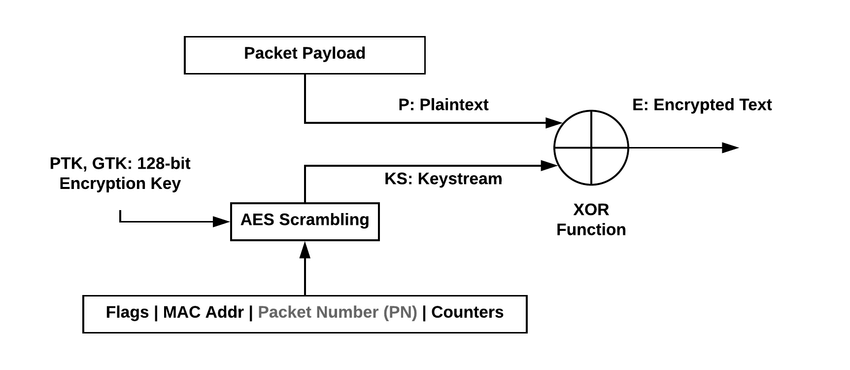
\includegraphics[width=15cm]{obrazky-figures/ccmp.png}
  \caption{Diagram šifrovaní CCMP \cite{kohlios2018comprehensive}.}
  \label{img:ccmp}
\end{figure}

Na začátku 4--fázové autentizace znají klient i přístupový bod SSID, Pairwise Master Key (PMK) a funkci Hash Message Authentication Protocol (HMAC) \cite{kohlios2018comprehensive}. Klient nejprve odešle přístupovému bodu žádost o připojení. Přístupový bod žádost potvrdí a poté vygeneruje a zašle tzv. ANonce -- jedná se o náhodně generovanou hodnotu k ověření toho, zda zná příjemce požadovanou informaci. Klient ji přijme a využije k vytvoření nové hodnoty (SNonce), kterou může přístupový bod otestovat. Pro vytvoření PTK pak klient spojí SNonce, ANonce a MAC adresy obou zařízení. Poté klient vygeneruje MIC a to za použití části PTK a následně zašle přístupovému bodu SNonce společně s MIC. Jelikož je při generování využito náhodných hodnot, pak je zajištěno, že hodnoty se pro každé sezení budou lišit.

V závislosti na využití sítě a na koncových uživatelích lze WPA využívat s různými ochrannými mechanizmy. Řadí se mezi ně \textit{WPA--Personal}, neboli WPA--PSK. Je používán pro domácnosti a malé kanceláře a nevyžaduje autentizační server. Pro sítě velkých společností je využíván \textit{WPA--Enterprise}, který však vyžaduje autentizační server -- zpravidla se jedná o server RADIUS.

I přes výrazné zlepšení oproti WEP však i WPA/WPA2 přináší několik bezpečnostních rizik, zejména:
\begin{itemize}
  \item{\textbf{Slabá hesla} -- předsdílené klíče využívané WPA a WPA2 jsou rizikové vzhledem k~možnosti prolomení slabých hesel. Metodou hrubé síly je tak možné slabé heslo prolomit. Nejnáchylnější na prolomení jsou často používaná hesla, které obsahuje většina slovníků hesel. Dobré heslo by mělo být náhodně generované a mít alespoň 16 znaků. Tento problém řeší příchod WPA3, které přichází s protokoly vyžadující interakci s~infrastrukturou sítě při každém pokusu o zadání hesla, což umožňuje nastavit časové limity na pokusy o uhádnutí hesla. V roce 2019 bylo však i ve standardu WPA3 objeveno několik nedostatků a došlo k tzv. Dragonblood útoku v průběhu kterého se podařilo prolomit heslo metodou hrubé síly \cite{vanhoef2020dragonblood}.}
  \item{\textbf{Nedostatečné zabezpečení do budoucna} -- pokud útočník získá předsdílený klíč, může dešifrovat obsah všech minulých i budoucích paketů v síti. WPA tedy chrání pouze před útočníkem, který nemá heslo. V moment, kdy útočník heslo získá už může v tichosti odchytávat pakety a za pomocí hesla je i dešifrovat. Tento problém je také řešen s příchodem WPA3.}
\end{itemize}

V lednu roku 2018 došlo k oznámení WPA3 jakožto náhrady za WPA2 a od 1. července 2020 je nutná certifikace WPA3 pro všechna nová zařízení označená jako Wi-Fi. Varianta WPA3-Personal využívá stále algoritmu CCMP-128, autentizaci za použití předsdílených klíčů (PSK) však nahrazuje za Simultaneous Authentication of Equals (SAE) -- čímž přináší ochranu proti reinstalaci klíčů v rámci KRACK exploitu. WPA3-Enterprise využívá k šifrování 256--bitový protokol Galois/Counter Mode Protocol (GCMP-256). WPA3 také implementuje lepší ochranu řídících rámců dle standardu IEEE 802.11w \cite{jonnalagadda2009method}. V tabulce \ref{table:wpa3} je uveden seznam nejpoužívanějších útoků na WPA2 a informace, zda přináší WPA3 zabezpečení proti těmto útokům. Tabulka \ref{table:wpa-compare} zobrazuje srovnání všech dostupných protokolů pro šifrování.
\begin{table}[htb]
\centering
\begin{tabular}{|c|c|}
\hline
\textbf{Útok} &\textbf{Řešení ve WPA3} \\ \hline
Deautentizace klienta & Ano \\ \hline
Slovníkový útok na zachycený handshake & Ano \\ \hline
Slovníkový útok na PMKID hash & Ano \\ \hline
Rouge Access Point & Částečně \\ \hline
Evil Twin & Ne \\ \hline
Dešifrovaní zachyceného handshake & Ano \\ \hline
KRACK exploit & Ano \\ \hline
ARP Spoofing & Částečně \\ \hline
SSL Stripping & Ne \\ \hline
DNS Spoofing & Ne \\ \hline
\end{tabular}
\caption{Přehled nejznámějších útoků a jejich řešení ve WPA3. Převzato z \cite{kohlios2018comprehensive}.}
\label{table:wpa3}
\end{table}

\begin{table}[htb]
\centering
\begin{tabular}{|c|c|c|c|}
\hline
\textbf{}                & \textbf{Šifrování}           & \textbf{Integrita dat} & \textbf{Autentizace}                        \\ \hline
\textbf{WEP}             & RC4 (40/104–bitový klíč)     & CRC                    & Sdílené klíče                     \\ \hline
\textbf{WPA-Personal}    & RC4 s TKIP (128–bitový klíč) & Michael                & PSK                     \\ \hline
\textbf{WPA-Enterprise}  & RC4 s TKIP (128–bitový klíč) & Michael                & 802.1x EAP                       \\ \hline
\textbf{WPA2-Personal}   & AES-CCMP (128–bitový klíč)   & CBC-MAC                & PSK                    \\ \hline
\textbf{WPA2-Enterprise} & AES-CCMP (128–bitový klíč)   & CBC-MAC                & 802.1x EAP                       \\ \hline
\textbf{WPA3-Personal}   & AES-CCMP (128–bitový klíč)   & CBC-MAC                & SAE \\ \hline
\textbf{WPA3-Enterprise} & AES-GCMP (256–bitový klíč)   & GMAC-256           & 802.1x EAP      \\ \hline
\end{tabular}
\caption{Srovnání všech dostupných protokolů pro šifrování.}
\label{table:wpa-compare}
\end{table}

\begin{figure}[htbp]
  \centering
  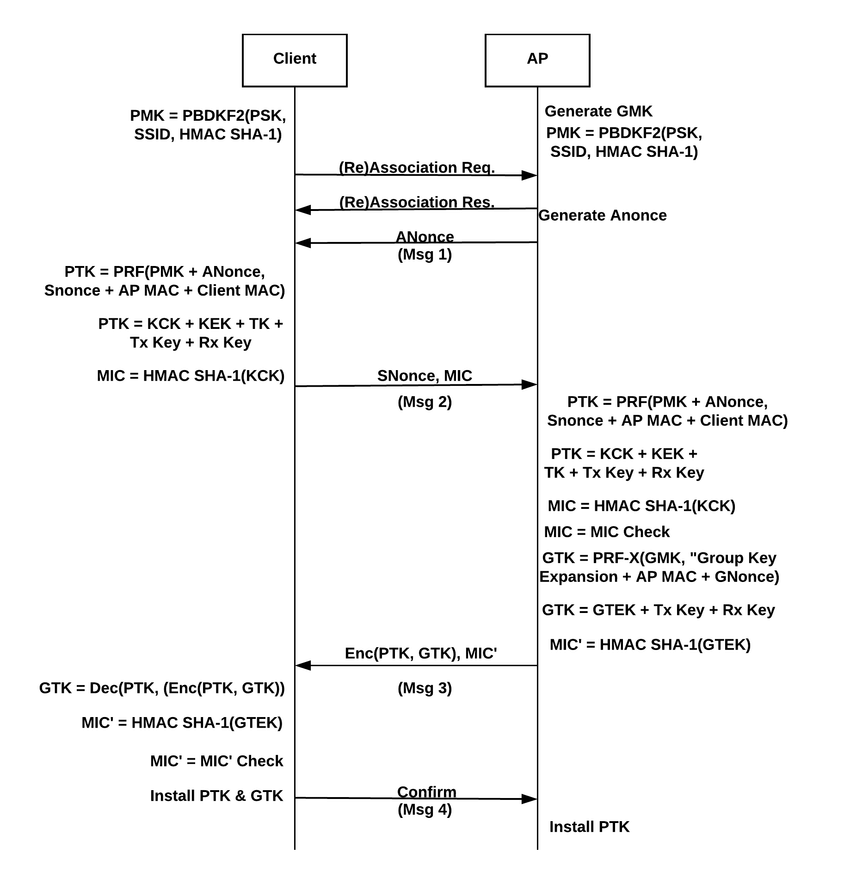
\includegraphics[width=15cm]{obrazky-figures/handshake.png}
  \caption{Diagram znázorňující 4-fázový handshake. Převzato z \cite{kohlios2018comprehensive}.}
  \label{img:handshake}
\end{figure}
%===============================================================================

\chapter{Prolomení zabezpečení Wi-Fi sítí} 
\label{prolomeni}
V této kapitole se podíváme na možnosti prolomení zabezpečení Wi-Fi sítí.

\section{Detekovatelnost útoků}
Pro odposlouchávání sítě je možné využít pasivního skenování a samotné odposlouchávání tak nemůže být detekováno. Odposloucháváním sítě může útočník získat informace o dané síti. Pokud je však obsah jednotlivých rámců šifrován, pro útočníka je jejich samotný obsah bezvýznamný. Útočník může také využít aktivního skenování či sondování a zasílat falešné rámce. K tomu je však již zapotřebí využití vysílače síťové karty a útok je tak již detekovatelný, navíc může dojít k lokalizaci místa síťové karty. Pokročilá moderní zařízení jsou konfigurována pro monitorování sítě a detekci neobvyklých událostí v síti -- obsahují jeden nebo více senzorů, které shromažďují údaje a je z nich možné získat například i MAC adresu potencionálního útočníka \cite{scarfone2012guide}. 

\subsection{Sondování sítě}
K aktivnímu sondování sítě se útočník uchyluje v moment, kdy informace z odposlechu sítě, tedy pasivního sondování, nejsou dostatečné. Oproti pasivnímu sondování je však to aktivní již v rámci sítě detekovatelné a útočník tak podstupuje jisté riziko. Aktivní sondování probíhá vytvořením falešných paketů s dotazy, díky kterým může útočník obdržet užitečné informace o síti. Určité bity v rámcích také označují, zda je odesílatelem stanice nebo přístupový bod -- útočník tak může získat přehled o všech stanicích komunikujících v síti.

Sondování probíhá nejčastěji sestavením falešných řídících rámců, pomocí kterých útočník může vyvolat nějakou akci přístupového bodu. Útočník může například zaslat přístupovému bodu podvržený deautentizační rámec s využitím MAC adresy klienta (viz obr.~\ref{img:deauth}) -- tím zapříčiní odpojení klienta od sítě. Klient se následně pokusí o znovupřipojení do sítě, čímž projde celým cyklem připojení do sítě (viz obr. \ref{img:komunikace}), který může útočník následně odposlechnout. Tento postup se používá například u prolamování WPA-PSK, jelikož před útokem musí útočník odposlechnout autentizační handshake. 

V průběhu sondování se využívá MAC spoofingu - jde o záměnu MAC adresy zdrojové stanice. U moderních síťových karet ji lze však poměrně jednoduše změnit. Díky změně MAC adresy může útočník získat neoprávněný přístup do sítě, nebo může změny adresy využít jako maskování. Existuje však i několik různých metod, jak MAC spoofing detekovat -- například za pomocí algoritmu používajícího PLCP hlavičky \cite{plcp}, nebo metodou náhodného lesa \cite{alotaibi2016new}. 

\subsubsection*{Získání SSID}
Běžně lze SSID přístupového bodu získat lehce odposlechem Beacon rámců. V případě, kdy je však SSID v Beacon rámcích skryto, pak by útočník musel čekat například na probe request či asociační žádost nějakého z klientů. Za využití aktivního sondování tak může útočník vytvořit vlastní probe request a z obdržené probe response získat samotné SSID přístupového bodu. Některé přístupové body však mohou být nastaveny tak, aby neodpovídaly na žádný probe request, který neobsahuje validní SSID. V takovém případě může útočník odeslat nějakému z klientů sítě deautentizační rámec s MAC adresou přístupového bodu. Tím vynutí odpojení klienta od sítě -- ten následně vyšle požadavek na opětovné připojení do sítě, který obsahuje i SSID přístupového bodu.


\subsection{Wardriving}
Wardriving je provázen za účelem získání a shromažďování informací o Wi-Fi sítích. Nejčastěji je prováděn v jedoucím vozidle za pomocí přenosného zařízení -- například notebooku či chytrého telefonu. Jde tedy o lokalizaci přístupových bodů a získání základních informací o těchto přístupových bodech za pohybu \cite{wardriving}. Útočník může Wardriving využít za účelem objevení špatně zabezpečených přístupových bodů. Lze z nich také zjistit aktuální využití různých druhů zabezpečení. V České republice funguje projekt Wifileaks, graf \ref{img:rozlozeni} zobrazuje rozložení zabezpečení\footnote{Data dostupná z webu Wifileaks \url{https://www.wifileaks.cz/statistika.php}}. Podobná analýza provedená i mimo Českou republiku uvádí mnohem vyšší podíl WPA-2\footnote{\url{https://securelist.com/research-on-unsecured-wi-fi-networks-across-the-world/76733/}}.

\begin{figure}[htbp]
  \centering
  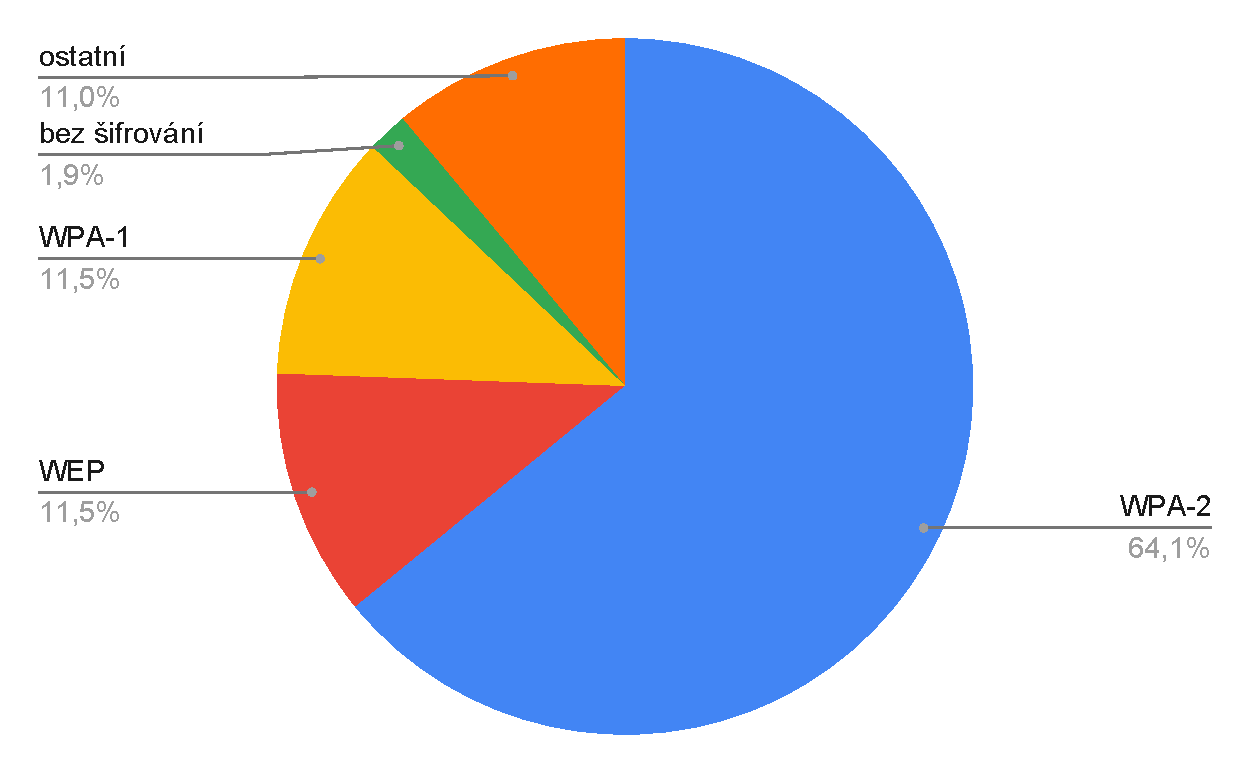
\includegraphics[width=15cm]{obrazky-figures/wifileaks.pdf}
  \caption{Přehled využití protokolů pro zabezpečení Wi-Fi sítí v České republice. Zobrazená data jsou z roku 2016.}
  \label{img:rozlozeni}
\end{figure}

Za zmínku stojí také Wardriving skupiny 0xDEADC0DE provedený v roce 2016 po Brně (viz obr~\ref{img:wardriving}). Účelem bylo zjistit, kolik se v Brně nachází přístupových bodů od společnosti UPC, které využívají základní konfigurace. Wardriving byl proveden v době, kdy bylo zjištěno, že lze v základní konfiguraci nových UPC routerů snadno vygenerovat heslo za pomocí SSID. Z projížďky autem, která trvala tři hodiny získali následující údaje~\cite{UPCPassword}:
\begin{itemize}
  \item{Zachyceno bylo 17516 unikátních přístupových bodů (BSSID).}
  \item{Celkem 2834 přístupových bodů neslo SSID ze základní konfigurace pro UPC a bylo tedy potencionálně snadno napadnutelných.}
\end{itemize}

\begin{figure}[htbp]
  \centering
  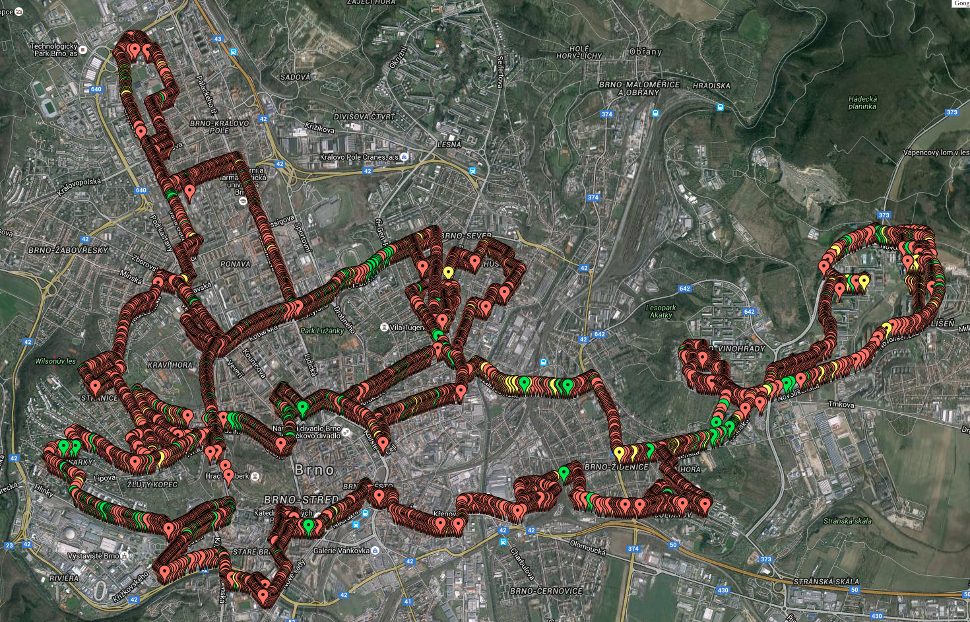
\includegraphics[width=15cm]{obrazky-figures/wardriving_map.png}
  \caption{Přehledná mapa zobrazující trasu Wardrivingu po Brně provedeného skupinou 0xDEADC0DE. Převzato z \cite{UPCPassword}.}
  \label{img:wardriving}
\end{figure}

\section{Metody útoků na Wi-Fi}

\subsection{Phishing}
Jeden z vůbec nejrychlejších způsobů, jak získat heslo od Wi-Fi sítě. Tento způsob cílí na samotné uživatele sítě a snaží se z~nich heslo vylákat. V moment, kdy se podaří útočníkovi z~uživatele heslo vylákat, pak už mu mnohdy nebrání nic v proniknutí do systému. Dosáhnout toho může například podstrčením falešné stránky na přihlášeni. 

\subsection{Cracking}
V případě, že sít využívá šifrování WEP či WPA se útočník uchyluje k prolomení klíče používaného pro šifrování. K prolomení samotného klíče lze využít několik různých metod a nástrojů. Jejich použití záleží především na konfiguraci daného přístupového bodu. Útok může být proveden jak aktivně -- za pomocí injektování paketů do provozu sítě, tak i pasivně pouhým pozorováním a odposloucháváním sítě. 

\subsubsection*{WEP Cracking}
Prolomení WEP je v dnešní době většinou otázkou pouze několika mála minut. Používá se k němu nejčastěji tzv. FMS útok. Útok spočívá v použití slabých inicializačních vektorů, odhadem zhruba 9 tisíc z 16 milionů inicializačních vektorů je považováno za slabé a může být při útoku využito. Pro prolomení 128-bitového klíče je potřeba zachytit zhruba dva miliony paketů \cite{stubblefield2002using}.

\subsubsection*{WPA/WPA2 Cracking}
Prolomení klíčů WPA a WPA2 je již složitější a při dobře nastaveném heslu mnohdy i~nemožné. Samotné prolamování hesla totiž vždy probíhá za pomocí metody tvrdé síly a slovníku hesel. Dobře sestrojený slovník hesel mnohdy rozhoduje o úspěchu či neúspěchu celého útoku. Nejobsáhlejší volně dostupný slovník s WPA hesly obsahuje osm miliard různých hesel\footnote{Ke stažení na adrese \url{https://github.com/berzerk0/Probable-Wordlists/}}. Tento slovník je sestaven především z uniklých hesel na internetu -- spoléhá tedy především na to, že uživatelé mnohdy používají stejné heslo pro více služeb.

První metoda využívá slabiny šifrování WPA-PSK u WPA i WPA2, kdy je při autentizaci proveden tzv. autentizační handshake, který má čtyři fáze. V průběhu této autentizace může útočník heslo zachytit a pokusit se ho prolomit. Nevýhodou této metody je však nutnost, aby byl k přístupovému bodu připojen alespoň jeden klient -- jinak není možné autentizaci zachytit. Samotnou autentizaci lze u klienta vyvolat zasláním deautentizace, což zapříčiní jeho následné opětovné připojení do sítě (viz obr. \ref{img:deauth}).

Druhá metoda byla objevena v roce 2018 a nevyžaduje žádného připojeného klienta. Tato metoda spočívá v tom, že útočník jednoduše požádá přístupový bod o PMKID (Pairwise Master Key Identifier), který obsahuje předsdílený klíč. Nutno podotknout, že metoda není univerzální -- ne všichni výrobci používají ve svých zařízeních PMKID.

Výstupem obou metod je šifrované heslo, které musí útočník prolomit. Prolomení probíhá stylem generování šifrovaných hesel ze slovníku hesel či metodou hrubé síly a jejich následným porovnáváním. Samotné prolomení hesla však už může útočník provádět offline mimo samotnou síť. Pokud selže slovníkový útok, pak je nutné přistoupit ke zkoušení náhodné kombinace hesel, šance na úspěch je poté velice malá. Moderní grafické karty zvládnou každou sekundu vyzkoušet zhruba sto tisíc kombinací \cite{alamanni2015kali}. Vyzkoušet tak všechny možné kombinace pro heslo o délce osmi znaků využívající všech ASCII znaků by trvalo více jak 24 dní. Pokud by heslo mělo délku deset znaku, celý proces by trval již 45 let. Pokud tedy síť využívá náhodně generovaného hesla o délce například 24 znaků, jeho prolomení je téměř nemožné.

Další metodou je neútočit na samotné šifrování WPA, ale podniknout tzv. WPS Pixie-Dust útok. WPS bylo vytvořeno za účelem usnadnění připojení nových zařízení do sítě. Mnohdy jde o tlačítko na routeru, které stačí zmáčknout a připojit tak do sítě všechna nová zařízení. WPS Pixie-Dust útok probíhá offline a není univerzální -- týká se jen určitých výrobců, včetně například Ralink, Realtek, a Broadcom \cite{mitnick2019art}. V závislosti na složitosti zvoleného WPS pinu může útok trvat vteřiny, ale i hodiny. 

\subsection{Man-in-the-middle}
Útok technikou man-in-the-middle (člověk uprostřed) spočívá v tom, že se útočník stane aktivním účastníkem komunikace a to bez vědomí účastníků této komunikace (viz obr. \ref{img:mitm}). Veškerá komunikace tak prochází přes samotného útočníka a ten ji může pozorovat a měnit obsah jednotlivých zpráv.

\begin{figure}[htbp]
  \centering
  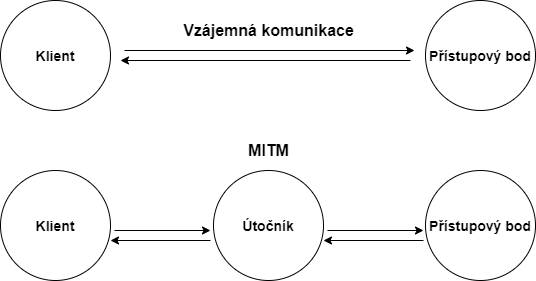
\includegraphics[width=10cm]{obrazky-figures/mitm.png}
  \caption{Pozice útočníka v komunikaci při man-in-the-middle útoku.}
  \label{img:mitm}
\end{figure}

Pozici man-in-the-middle může útočník využít více způsoby. Nejčastější využití je úprava řídících rámců. Celý útok může být veden následovně \cite{beaver2015hacking}:
\begin{enumerate}
  \item{Útočník nalezne klienta, který aktivně komunikuje s přístupovým bodem. Získá RF kanál a MAC adresu tohoto klienta.}
  \item{Útočník odešle klientovi deautentizační rámec, čímž vynutí u klienta odpojení od přístupového bodu.}
  \item{Útočník zprovozní podvržený přístupový bod, který se bude tvářit jako ten původní -- bude využívat stejné SSID a MAC adresu.}
  \item{Klient se následně snaží znovu připojit do sítě. Útočník má poměrně velké šance, že se klient připojí právě do jeho podvržené sítě.}
  \item{Útočník se následně připojí na pravý přístupový bod. Díky tomu se právě stal útočník prostředníkem celé komunikace.}
\end{enumerate}

\section{Známé útoky na Wi-Fi sítě}
Existuje řada známých útoků, které využívají zejména chyby v používaných protokolech, či nedostatky ve standardech jednotlivých protokolů \cite{kohlios2018comprehensive}.

\subsection{Deautentizace klienta}
Již zmiňovaný útok, který je hojně využíván. Při vstupu do sítě musí klient projít procesem autentizace a přístupový bod klienta informuje o úspěchu či neúspěchu tohoto procesu. Pokud je provedena celá autentizace, včetně 4-fázového handshake, úspěšně, pak si mohou klient a přístupový bod posílat vzájemně šifrovaná data. Samotný útok spočívá v tom, že útočník použije MAC adresu klienta sítě a odešle přístupovému bodu deautentizační rámce s touto MAC adresou, čímž dojde k odpojení klienta od sítě (viz obr. \ref{img:deauth}). 
\begin{figure}[htbp]
  \centering
  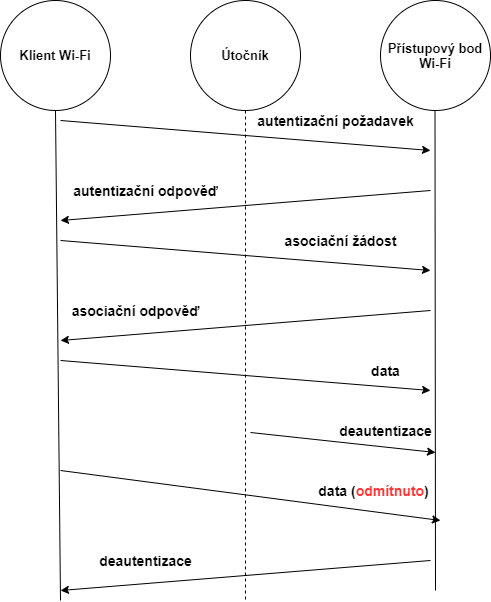
\includegraphics[width=10cm]{obrazky-figures/deauth.png}
  \caption{Znázornění provedení deautentizace klienta v síti.}
  \label{img:deauth}
\end{figure}

\subsection{Slovníkový útok na zachycený handshake}
Útočník nejprve odposlouchává síť a snaží se zachytit 4-fázový handshake mezi klientem a přístupovým bodem. Po jeho zachycení má útočník potřebné informace pro provedení offline slovníkového útoku. Na tomto heslu je založena derivační funkce (PBKDF2) v PSK. Útočník tak provede stejný proces, jako při 4-fázovém handshake (viz obr. \ref{img:handshake}), získá MIC a PTK, díky čemuž si může ověřit, zda-li se daná položka ze slovníku shoduje s heslem~\cite{kumkar2012vulnerabilities}. 

\subsection{Slovníkový útok na hash PMKID}
V roce 2018 byla odhalena nová metoda offline slovníkového útoku na Wi-Fi sítě. Tento druh útoku byl odhalen při zkoumání možných útoků na WPA3 -- jde o útok, který nevyžaduje zachycení autentizačního handshake a tedy nevyžaduje nutnost připojeného klienta v síti. Útok zneužívá protokolu Extensible Authentication Protocol (EAP), konkrétně jednoho z~jeho rámců -- jedná se o tzv. EAPOL rámec. Ten obsahuje hodnotu PMKID, která je tvořena následovně:
\begin{equation}
PMK_{ID}=H(PMK,PMK_{Name}|MAC_{AP}|MAC_{STA})
\end{equation}
Skládá se tedy z klíče PMK, PMK názvu a MAC adresy přístupového bodu a klienta. Útočník tak může sám lehce, za použití hesla ze slovníku, sestrojit PMKID hash a porovnat ho s hodnotou PMKID v zachyceném EAPOL rámci. 

\subsection{Evil Twin útok}
Útok, při kterém útočník vytvoří přístupový bod totožný s tím skutečným -- bude tedy obsahovat stejné SSID a bude fungovat na stejném kanálu. Pokud zná útočník i heslo ke skutečnému přístupovému bodu, pak bude mít podvržený přístupový bod i stejné heslo. Následně bude útočník doufat, že někteří uživatelé se připojí k jeho vytvořenému přístupovému bodu, místo připojení k tomu skutečnému. Podvržený přístupový bod mnohdy nabízí v daném místě lepší připojení a tak se většina uživatelů připojí právě k němu. Útočník tak získá pozici man-in-the-middle (MITM). Veškerý provoz bude útočník směřovat dále, mnohdy ke skutečnému přístupovém bodu a samotný uživatel tak nic nepozná. 

Útočník také může po zprovoznění podvrženého přístupového bodu vyvolat deautentizaci klientů ve skutečné síti a tím celý proces připojení klientů do podvržené sítě urychlit. Spousta zařízení se navíc do podvržené sítě (díky stejnému SSID, heslu a lepší kvalitě připojení) připojí automaticky. 

\subsection{KRACK Exploit}
V roce 2016 objevili Mathy Vanhoef a Frank Piessens vážné nedostatky ve standardu Wi-Fi sítí\footnote{Implementace KRACK exploitu je dostupná na \url{https://github.com/vanhoefm/krackattacks-scripts}}. Útok je prováděn proti 4-fázové autentizaci protokolu WPA2. Provedením tohoto útoku donutí útočník klienta k reinstalaci již používaného klíče. 

Po přijetí třetí zprávy 4-fázové autentizace provede klient instalaci klíče. Po instalaci klíče je tento klíč využíván k šifrování a dešifrování všech dat posílaných mezi klientem a~přístupovým bodem. Jelikož však může dojít ke ztrátě třetí zprávy, přístupový bod ji zasílá opakovaně až do chvíle, kdy obdrží odpověď od klienta pro potvrzení doručení této zprávy. V důsledku toho může klient obdržet zprávu vícekrát a při každém obdržení této zprávy dojde k instalaci stejného klíče -- zároveň s instalací klíče dojde k obnovení přírůstkového čísla paketu (tzv. nonce) a čítače opakování. Útočník může toto obnovení vynutit shromažďováním a~následným opakováním třetí zprávy. Poté může dojít k napadení šifrovacího protokolu a~útočník tak může například dešifrovat obsah paketů \cite{vanhoef-ccs2017}. 

\subsection{Kr00k Exploit}
Jedná se o bezpečnostní chybu objevenou v roce 2019\footnote{Implementace Kr00k exploitu je dostupná na \url{https://github.com/hexway/r00kie-kr00kie}}. Chyba se týká všech zařízení, které využívají čipy od společností Broadcom a Cypress FullMac. Podle společnosti ESET, která chybu odhalila, se tato chyba týká více jak miliardy zařízení po celém světě. Chyba umožňuje prolomení WPA2 využívajícího šifrování CCMP.

V moment, kdy dojde u klienta ke zrušení asociace s přístupovým bodem, je klíč se sezením (TK), který je uložen na kontroléru síťového rozhraní (WNIC) čipu Wi-Fi vyprázdněn -- nastaven na hodnotu nula. Jedná se o běžnou věc, jelikož se po zrušení asociace již neočekává přenos dalších dat. Bylo však zjištěno, že všechny datové rámce, které zůstaly v~čipech Tx bufferu, byly přenášeny poté, co byly zašifrovány tímto nulovým klíčem \cite{CVE-2019-15126}. Obrázek~\ref{img:kr00k} znázorňuje rámce šifrované nulovým heslem po odpojení klienta.

\begin{figure}[htbp]
  \centering
  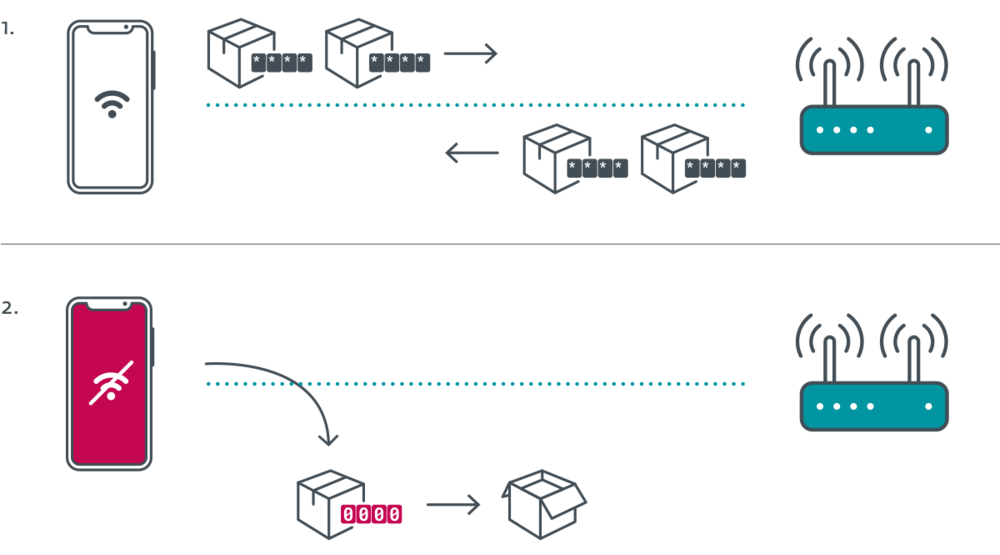
\includegraphics[width=14.7cm]{obrazky-figures/kr00k.png}
  \caption{Znázornění Kr00k exploitu. Převzato z \cite{CVE-2019-15126}.}
  \label{img:kr00k}
\end{figure}

\subsection{ARP spoofing}
Tento útok zneužívá protokolu ARP, který je využíván k mapování IP adresy klienta na jeho MAC adresu. Klienti mají tabulku ARP, která obsahuje IP adresy všech ostatních klientů v síti a k nim přiřazené MAC adresy. Při vstupu klienta do sítě dojde k vyslání broadcastu s žádostí o identifikaci ostatních zařízení v síti. Ostatní účastníci zašlou odpověď obsahující jejich IP a MAC adresy. Protokol ARP po obdržení těchto odpovědí naplní tabulku ARP. Komunikaci v rámci protokolu ARP zobrazuje obrázek \ref{img:arp}.

Problém tohoto protokolu je však fakt, že nevyužívá žádné autentizace ani ověření. Útočník tak jednoduše může sestrojit vlastní ARP odpovědi a rozeslat je klientům v síti. Klienti odpovědi přijmou (a to i v případě, že nezasílali žádný dotaz) a zapíšou změny do~tabulky ARP. Útočník tak může libovolnou IP adresu označit jako IP adresu jeho zařízení, tedy přiřadit k libovolné IP adrese svoji MAC adresu. Veškerý provoz na danou IP adresu ze strany daného klienta pak bude tedy směrován právě k útočníkovi.
\begin{figure}[htbp]
  \centering
  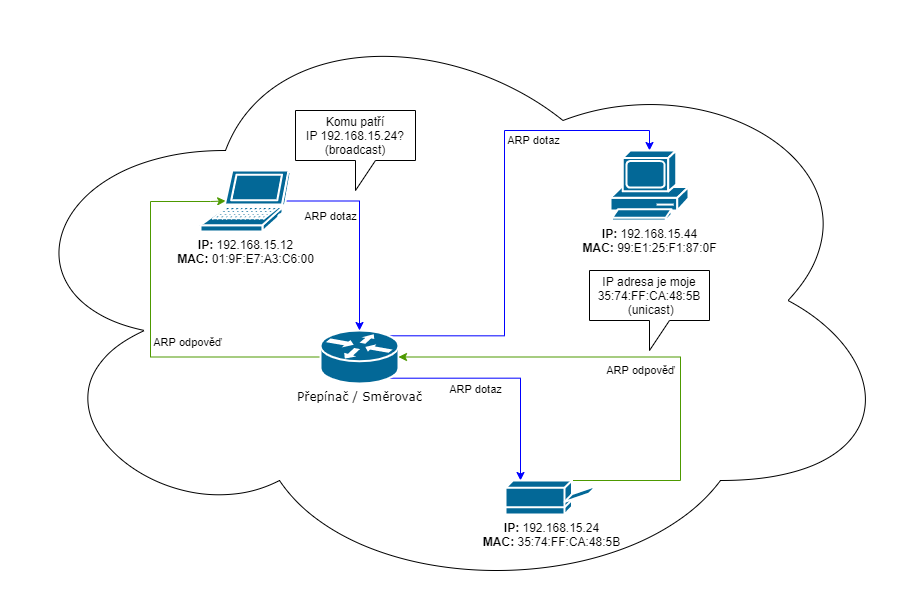
\includegraphics[width=14.7cm]{obrazky-figures/arp.png}
  \caption{Komunikace mezi jednotlivými stanicemi v síti při vyslání ARP dotazu.}
  \label{img:arp}
\end{figure}

\subsection{SSL Stripping}
Pokud se útočník dostane do pozice man-in-the-middle, pak může provést útok metodou SSL Stripping. Když se klient připojí k webové stránce za pomocí protokolu Hypertext Transfer Protocol (HTTP), pak může útočník celý proces plně pozorovat a případně ho měnit. Tomu zabraňuje protokol HTTPS, který je kombinací protokolů HTTP a SSL a zajišťuje šifrování přenesených dat protokolem SSL. Pokud se tedy klient připojuje na webové stránky využívající protokol HTTPS, pak jsou zachycená data pro útočníka bezcenná. 

Za pomocí útoku zvaného SSL Stripping však může útočník zařídit, aby k webu klient přistupoval přes nezabezpečený HTTP protokol. Pokud klient přistoupí na webovou stránku využívající HTTPS, útočník změní požadavek z HTTPS protokolu na HTTP. Útočník pak sám s webem naváže HTTPS spojení. Vytvoří se tedy dvě spojení, zabezpečené mezi webem a útočníkem a nezabezpečené mezi klientem a útočníkem. Útočník tak může jednoduše pozorovat aktivitu klienta, která pro něj v tento moment není nijak šifrovaná -- může tak odcizit jeho přihlašovací údaje, údaje od platebních karet apod. Uváděny jsou pouze chyby, které může útočník využít při útoku za účelem proniknutí do sítě.

\section{Chyby jednotlivých zařízení}
Jak již bylo zmíněno, mnohdy se chyb v zabezpečení dopouští samotní výrobci zařízení. Následující sekce si bere za úkol prozkoumat zařízení používaná v České republice a nalézt případné chyby v nich. Výběr obsahuje routery, které se umístily v prvním čtvrtletí roku 2020 v České republice jako nejprodávanější. Také obsahuje zařízení dodávaná společnostmi UPC a O2 koncovým zákazníkům. Uvedena jsou pouze zařízení, u kterých byla objevena nějaká závažná chyba, kterou lze využít, aniž by musel útočník být do sítě připojen. Detaily jednotlivých chyb a možnosti jejich zneužití jsou uvedeny v přiložených zprávách, na které odkazují v poznámce pod čarou.

\subsection*{CBN CH7465LG}
Router dodávaný společností UPC. V rámci velké zprávy o zabezpečení tohoto zařízení provedeného týmem bezpečnostních expertů z Maďarska došlo k odhalení několika chyb v~samotném zařízení\footnote{Zpráva dostupná na \url{www.search-lab.hu/media/Compal_CH7465LG_Evaluation_Report_1.1.pdf}}. Mimo jiné obsahuje i chyby umožňující:
\begin{itemize}
  \item{odepření služby (DoS útok),}
  \item{možnost injektování vlastních příkazů,}
  \item{přístup k rozhraní pro zálohy a tovární obnovení routeru bez autentizace.}
\end{itemize}
Využitím poslední uvedené chyby se útočník může dostat k zálohám nastavení routeru, kde nalezne veškerou konfiguraci routeru, včetně hesla použitého pro šifrování.

\subsection*{TECHNICOLOR TC7200}
Další z řady routerů dodávaných společností O2. Toto zařízení také obsahuje chybu v přístupu k zálohám routeru. Zálohy jsou šifrovány algoritmem AES za pomocí klíče použitého při autentizaci. K zálohám se však dá přistupovat bez autentizace, to způsobí, že nelze nastavit heslo pro šifrování a zálohu lze tak snadno dešifrovat za pomocí prázdného klíče\footnote{Podrobný popis chyby na \url{https://www.exploit-db.com/exploits/40157}}.

\subsection*{CISCO EPC3925}
Opět zařízení dodávané společností O2. V zařízení byla objevena velmi závažná chyba umožňující vzdálenému útočníkovi způsobit přetečení zásobníku a následně spustit libovolný kód. Příčinou je špatná vstupní validace HTTP požadavků. Chybu tak může útočník využít zasláním sestrojeného HTTP požadavku\footnote{Podrobnější informace na \url{https://tools.cisco.com/security/center/downloadPDF.pdf}}.

\subsection*{ZTE ZXHN H168N}
Tento router dodává společnost UPC. Obsahuje chybu ve zpracování HTTP požadavků, který umožňuje útočníkovi vytvořit speciální HTTP požadavek a tím získat kontrolu nad zařízením\footnote{Popis chyby na \url{https://fortiguard.com/encyclopedia/ips/48669}}.

\subsection*{TP-Link Archer MR200 a MR6400}
Oba routery jsou dodávány společností UPC. Chyba byla objevena roku 2019 bezpečnostními experty z IBM. Znovu se jedná o chybu při zpracovávání HTTP požadavků. Při zneužití chyby může útočník získat kontrolu nad konfigurací routeru\footnote{\url{https://securityintelligence.com/posts/tp-link-archer-router-vulnerability-voids-admin-password-can-allow-remote-takeover/}}.

\subsection*{Xiaomi Mi Router 4A}
Druhý nejprodávanější router v prvním čtvrtletí roku 2020 v českých obchodech. Na internetu je volně dostupný nástroj\footnote{Nástroj dostupný na \url{https://github.com/acecilia/OpenWRTInvasion}}, který dokáže využít chybu v tomto zařízení a dát útočníkovi plný přístup do konzole, ze které může spouštět libovolné příkazy. 

\chapter{Existující nástroje pro prolomení zabezpečení Wi-Fi sítí}
\label{nastroje}
Tato kapitola uvádí výčet nejpoužívanějších nástrojů pro útoky na Wi-Fi sítě. Dále obsahuje ukázku jejich použití a následní porovnání těchto nástrojů.

\section{Přehled nástrojů}
\subsection{Aircrack-ng}
\label{aircrack}
Aircrack-ng\footnote{Ke stažení na adrese \url{https://www.aircrack-ng.org/}} je kompletní nástroj nabízející útoky na Wi-Fi sítě včetně možnosti prolamování hesel WEP a WPA PSK. Dostupný je pro Linuxové distribuce i systémy Windows. Nástroj nabízí následující možnosti:
\begin{itemize}
  \item{\textbf{Monitorování} -- zachytávání přenášených paketů a možnost jejich exportu.}
  \item{\textbf{Útok} -- vytváření podvržených paketů, vytváření podvržených přístupových bodů a~další.}
  \item{\textbf{Testování} -- zjištěni kompatibility síťové karty a ovladačů pro jednotlivé útoky.}
  \item{\textbf{Prolamování hesel} -- WEP a WPA PSK používaného ve WPA a WPA2.}
\end{itemize}

Před použitím nástroje je nutné se ujistit, že použitá síťová karta umí injektovat pakety. To se dá zjistit provedením takzvaného injektivního testu. Celý test také může přinést zajímavé informace -- jelikož výsledkem testu je i seznam všech přístupových bodů v okolí, které odpověděly na probe request. Po spuštění nástroje nejprve dojde k vyslání probe requestů za pomocí broadcastu. V moment, kdy obdrží program od nějakého přístupového bodu odpověď, pak tuto informaci zobrazí -- tím jsme si ověřili, že naše síťová karta umožňuje injektování paketů. V průběhu také odposlouchává Beacon pakety a všechny přístupové body získané z nich také umístí do celkového seznamu. Poté každé nalezené přístupové stanici odešle třicet probe requestů. Výsledkem je počet obdržených odpovědí, který indikuje kvalitu spojení s daným přístupovým bodem. Výstup celého testu může být následující:
\begin{lstlisting}[language=bash]
$ aireplay-ng --test wlp6s0
19:52:31  Trying broadcast probe requests...
19:52:31  Injection is working!
19:52:33  Found 2 APs

19:52:33  Trying directed probe requests...
19:52:33  80:02:9C:30:D4:08 - channel: 2 - 'Sopfovi'
19:52:33  Ping (min/avg/max): 1.570ms/11.680ms/33.918ms Power: -48.43
19:52:33  30/30: 100%

19:52:33  14:CC:20:93:D5:E2 - channel: 2 - 'TP-LINK_93D5E2'
19:52:34  Ping (min/avg/max): 7.476ms/21.720ms/25.911ms Power: -54.67
19:52:34  30/30: 100%
\end{lstlisting}
Z odpovědi můžeme vyčíst, že test proběhl úspěšně. Naše síťová karta tak podporuje injektování paketů. V okolí jsme nalezli dva přístupové body. U obou je kvalita spojení 100\%. Z~testu jsme také získali MAC adresy a kanál přístupových bodů.

\subsubsection*{WEP Cracking}
Před samotným útokem je potřeba ověřit, že jsme schopni útok podniknout, potřebujeme k tomu:
\begin{enumerate}
  \item{Síťovou kartu a ovladače podporující injektování paketů -- lze ověřit injektivním testem.}
  \item{K síti na kterou útočíme musí být připojen alespoň jeden klient -- jelikož tento postup vyžaduje získání ARP odpovědi.}
  \item{K přístupovému bodu musíme mít kvalitní připojení a musíme být schopni přijímat i~odesílat pakety -- lze též ověřit injektivním testem.}
\end{enumerate}

Pokud jsme našli vhodnou síť a přístupový bod, můžeme se pustit do samotného útoku. Pro prolomení WEP klíče zvoleného přístupového bodu bude potřeba shromáždit velké množství inicializačních vektorů. Toho můžeme dosáhnout pouhým odposloucháváním sítě. Pro zrychlení procesu však nástroj provede injekci těchto paketů. Celý útok se odehrává v~pěti krocích:
\begin{enumerate}
  \item{\textbf{Přepnutí bezdrátového rozhraní do monitorovacího módu na kanálu přístupového bodu} -- tím zajistíme, že naše síťová karta bude odposlouchávat každý paket na daném kanálu. V běžném módu by totiž karta přijímala pouze pakety určené vašemu zařízení. Monitorovací mód na síťovém rozhraní wlp6s0 můžeme spustit následujícím příkazem:
\begin{lstlisting}[language=bash]
airmon-ng start wlp6s0 2
\end{lstlisting}
  }
  \item{\textbf{Zachytávání inicializačních vektorů} -- stačí BSSID cílového přístupového bodu a~jeho kanál. Po spuštění je proces plně automatizovaný a program nás informuje o jeho procesu formou informací o celkovém počtu zachycených paketů. Program spouštíme následovně:
\begin{lstlisting}[language=bash]
airodump-ng -c 2 --bssid 14:CC:20:93:D5:E2 -w vystup wlp6s0
\end{lstlisting}
  }
  \item{\textbf{Provedení autentizace s přístupovým bodem} -- provedením falešné autentizace zapříčiníme, že přístupový bod bude přijímat pakety přicházející z našeho zařízení. Pro provedení falešné autentizace budeme potřebovat navíc i MAC adresu našeho zařízení a provedeme ji následujícím příkazem:
\begin{lstlisting}[language=bash]
aireplay-ng -1 0 -e "TP-LINK_93D5E2" -a 14:CC:20:93:D5:E25 -h D4-6E-0E-11-AA-31
\end{lstlisting}
  }
  \item{\textbf{Odposlech ARP požadavků a jejich injekce} -- následně se můžeme pustit do odposlouchávání ARP požadavků. V moment, kdy spuštěný program zachytí jakýkoliv ARP požadavek, ihned provede jeho injekci do sítě. Celou operaci spustíme následovně:
\begin{lstlisting}[language=bash]
aireplay-ng -3 -b 14:CC:20:93:D5:E25 -h D4-6E-0E-11-AA-31 wlp6s0
\end{lstlisting}
  }
  \item{\textbf{Získání WEP klíče} -- pro samotné prolomení klíče můžeme využít dvě metody a to metodu PTW nebo FMS/Korekovu metodu. V základu je použita PTW metoda, použití druhé metody můžeme dosáhnout použitím přepínače \textbf{-K}. Po spuštění programu dojde následně v rámci několika sekund k vygenerování používaného WEP klíče. 
\begin{lstlisting}[language=bash]
aircrack-ng -b 14:CC:20:93:D5:E25 vystup*.cap
\end{lstlisting}
  }
\end{enumerate}

Za použití Aircrack-ng je prolomení WEP opravdu snadné. Nejvíce času zabere shromažďování inicializačních vektorů. Po shromáždění dostatku inicializačních vektorů je prolomení samotného hesla otázkou několika mála minut.

\subsubsection*{WPA/WPA2 Cracking}
Aircrack-ng podporuje pouze prolamování hesel u WPA-PSK, tedy WPA/WPA2 využívajících předsdílených klíčů. Zatímco u WEP lze k urychlení celého procesu využít statických metod, u WPA probíhá celý proces metodou hrubé síly. V použití nástroje pro WPA a~WPA2 není vzhledem k téměř stejné metodě autentizace žádný rozdíl. Samotný klíč může mít délku 8 až 64 znaků a tak jsou šance na prolomení mnohdy minimální. Úspěch prolomení je tak většinou pouze u slovníkových hesel. Útok lze spustit ve čtyřech krocích:
\begin{enumerate}
  \item{\textbf{Přepnutí bezdrátového rozhraní do monitorovacího módu na kanálu přístupového bodu} -- stejné jako u WEP:
\begin{lstlisting}[language=bash]
airmon-ng start wlp6s0 2
\end{lstlisting}
  }
  \item{\textbf{Zachytávání autentizačního handshake} -- cílem tohoto kroku je zachytit autentizační handshake s přístupovým bodem, na který útočíme. Zachytání spustíme příkazem:
\begin{lstlisting}[language=bash]
airodump-ng -c 2 --bssid 14:CC:20:93:D5:E2 -w vystup wlp6s0
\end{lstlisting}
  }
  \item{\textbf{Provedení de-autentizace klienta} -- tento krok slouží pouze jako urychlení pro zachycení autentizačního handshake. Provést ho můžeme následovně:
\begin{lstlisting}[language=bash]
aireplay-ng -0 1 -a 14:CC:20:93:D5:E2 -c 2F-26-B6-F1-C1-47 wlp6s0
\end{lstlisting}
  }
  \item{\textbf{Spuštění útoku} -- následně můžeme již spustit samotný útok. Na vstup zadáme slovník hesel -- nástroj pak postupně vezme každé heslo ze slovníku a vyzkouší jej. Útok se spouští příkazem:
\begin{lstlisting}[language=bash]
aircrack-ng -w hesla.txt -b 14:CC:20:93:D5:E2 vystup*.cap
\end{lstlisting}
  }
\end{enumerate}
Rychlost celého útoku záleží na výpočetním výkonu použité jednotky a na kvalitě hesla, které musí být obsaženo ve slovníku.

\subsection{Hcxtools a Hashcat}
Hcxtools je volně dostupný\footnote{Ke stažení na adrese \url{https://github.com/ZerBea/hcxtools}} nástroj pro Linuxové distribuce. Využívá se zejména při PMKID útoku na WPA-PSK v kombinaci s nástroji z programu Aircrack-ng. 

Pro provedení PMKID útoku je nejprve nutné přepnout síťovou kartu do monitorovacího módu za využití nástroje airmon-ng (viz kapitola \ref{aircrack}). Poté postupujeme následovně:
\begin{enumerate}
  \item{\textbf{Zachytávání PMKID} -- za pomocí nástroje hcxdumptool začneme zachytávat PMKID. V moment, kdy jich zachytíme dostatek můžeme program ukončit. Celou operaci spustíme následovně:
\begin{lstlisting}[language=bash]
hcxdumptool -i wlp6s0mon -o vysledek.pcapng --enable__status=1
\end{lstlisting}
  }
  \item{\textbf{Převedení PCAPNG formátu} -- následně je potřeba převést výstupní formát za pomocí nástroje Hxcpcaptool:
\begin{lstlisting}[language=bash]
hcxpcaptool -E essidlist -I identitylist -U usernamelist -z vysledek vysledek.pcapng
\end{lstlisting}
  }
  \item{\textbf{Prolamování hesla} -- po převedení výstupních dat se již můžeme pustit do samotného prolamování hesla. Pokusíme se tedy heslo prolomit za pomocí slovníku hesel:
\begin{lstlisting}[language=bash]
hashcat vysledek --force 'hesla.txt' -w 4 -a 0 -m 16800 --kernel-accel=1
\end{lstlisting}
  }
\end{enumerate}

Provedli jsem tak útok na WPA-PSK bez nutnosti, aby byl k síti připojený nějaký klient. Úspěch při prolomení samotného hesla je pravděpodobný opět však jen v případě slabého hesla. 

\subsection{Airgeddon}
Airgeddon tvoří balíček nástrojů pro útoky na bezdrátové sítě. Je volně dostupný pro platformu Linux\footnote{Ke stažení na adrese \url{https://github.com/v1s1t0r1sh3r3/airgeddon}}. Celý nástroj je lehce ovladatelný přes textové uživatelské rozhraní. 

Při spuštění programu dojde ke zkontrolování dostupných nástrojů na aktuálním systému (viz obr. \ref{img:airgeddon-packages}). Následně pomocí přehledného menu zvolíme požadovaný typ útoku (viz obr. \ref{img:airgeddon-menu}). Nástroj nabízí především následující možnosti:
\begin{itemize}
  \item{\textbf{Přepínání módu síťového rozhraní} -- možnost vypínat a zapínat monitorovací mód.}
  \item{\textbf{WEP útok} - všechny dostupné metody v jednom.}
  \item{\textbf{WPS útoky:} -- Pixie Dust útok, útok na WPS PIN metodou hrubé síly, útok na základě veřejně dostupných WPS pinů.}
  \item{\textbf{Offline WPA/WPA2 cracking}}
  \item{\textbf{Evil Twin útoky}}
\end{itemize}

\begin{figure}
\centering
\begin{subfigure}{.5\textwidth}
  \centering
  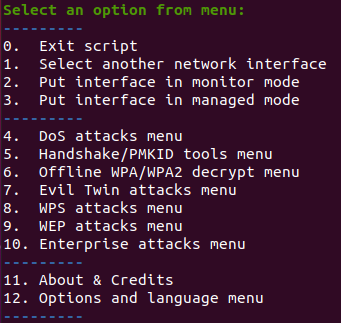
\includegraphics[width=.8\linewidth]{obrazky-figures/airgeddon-menu.png}
  \caption{Hlavní nabídka}
  \label{img:airgeddon-menu}
\end{subfigure}%
\begin{subfigure}{.5\textwidth}
  \centering
  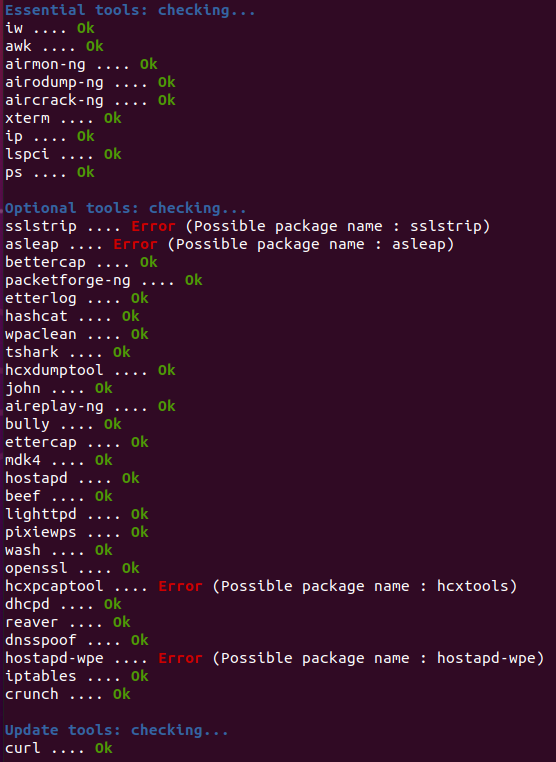
\includegraphics[width=.9\linewidth]{obrazky-figures/airgeddon-packages.png}
  \caption{Kontrola dostupných balíčků}
  \label{img:airgeddon-packages}
\end{subfigure}
\caption{Ukázka nástroje Airgeddon.}
\label{img:airgeddon}
\end{figure}

\subsection{Besside-ng}
Jedná se o automatizovaný nástroj pro crackování WEP a WPA/WPA2. Nástroj se automaticky snaží prolomit veškerou komunikaci v okolí šifrovanou za pomocí WEP. Zároveň zachytává WPA handshake pakety, které lze následně použít při offline crackování. Také se ale snaží i online prolomení WPA klíče za pomocí různých online služeb -- uvádí se úspěšnost zhruba 18\%. Nástroj se spouští za pomocí příkazu:
\begin{lstlisting}[language=bash]
besside-ng wlp6s0
\end{lstlisting}
Následně dojde k postupnému skenování všech kanálů. Pokud chceme skenovat pouze určitý kanál, můžeme toho docílit za pomocí přepínače \textbf{-c}. Také můžeme útočit jen na BSSID určitého přístupového bodu, stačí použít přepínač \textbf{-b}.

\subsection{LAZY skript}
Další z dostupných balíčků pro útoky na Wi-Fi. Kód tohoto nástroje je volně dostupný\footnote{Ke stažení na adrese \url{https://github.com/arismelachroinos/lscript}}. Opět obsahuje jednoduché a přehledné textové menu (viz obr. \ref{img:lazy}). Nástroj shlukuje nejpoužívanější nástroje a nabízí jejich jednoduché použití, navíc nabízí i možnost ovládat nastavení síťových adaptérů. Nástroj nabízí provedení především následujících útoků:
\begin{itemize}
  \item{\textbf{WEP} -- zachycení inicializačních vektorů a prolomení hesla.}
  \item{\textbf{WPS pin} -- metodou hrubé síly, či za pomocí databáze nejpoužívanějších pinů.}
  \item{\textbf{WPA handshake} -- útok na WPA/WPA2 handshake.}
  \item{\textbf{Email spoofing}}
\end{itemize}

\begin{figure}[htbp]
  \centering
  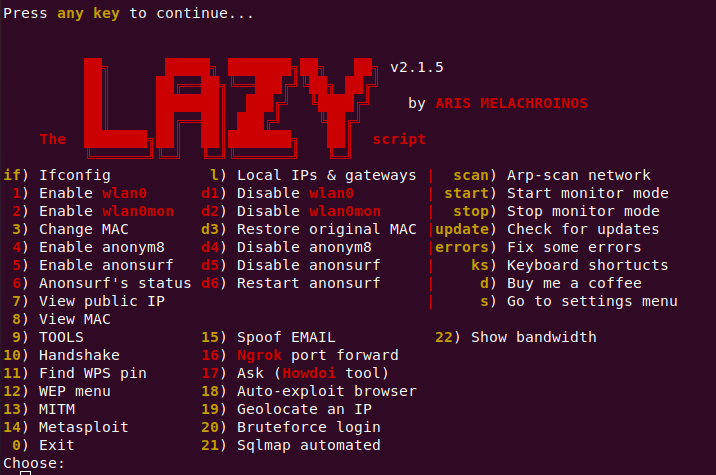
\includegraphics[width=14.7cm]{obrazky-figures/lazy.png}
  \caption{Hlavní nabídka LAZY skriptu.}
  \label{img:lazy}
\end{figure}

\subsection{Wifite2}
Další z řady jednoduchých a plně automatizovaných nástrojů. Nástroj nabízí volně dostupný kód pro platformu Linux\footnote{Ke stažení na adrese \url{https://github.com/derv82/wifite2}}. Po spuštění provede skenování daného kanálu:
\begin{lstlisting}[language=bash]
wifite -c2
\end{lstlisting}
Z dostupných přístupových bodů následně zvolíme ten, na který chceme útočit (viz obr.~\ref{img:wifite}). O vše ostatní se už postará nástroj. Za pomocí přepínače \textbf{-b} můžeme také rovnou zvolit BSSID přístupového bodu, na který chceme útočit.

Nástroj sám zvolí nejlepší metodu útoku a pokusí se prolomit heslo do zvolené sítě. Používá k tomu následující metody:
\begin{itemize}
  \item{\textbf{WPS} -- Offline útok Pixie-Dust.}
  \item{\textbf{WPS} -- Online útok metodou hrubé síly.}
  \item{\textbf{WPA handshake} -- Zachycení 4-fázové handshake autentizace a následný offline cracking.}
  \item{\textbf{WPA PMKID} -- Zachycení PMKID hashe a následný offline cracking.}
  \item{\textbf{WEP} -- řada nejpoužívanějších útoků.}
\end{itemize}

\begin{figure}[htbp]
  \centering
  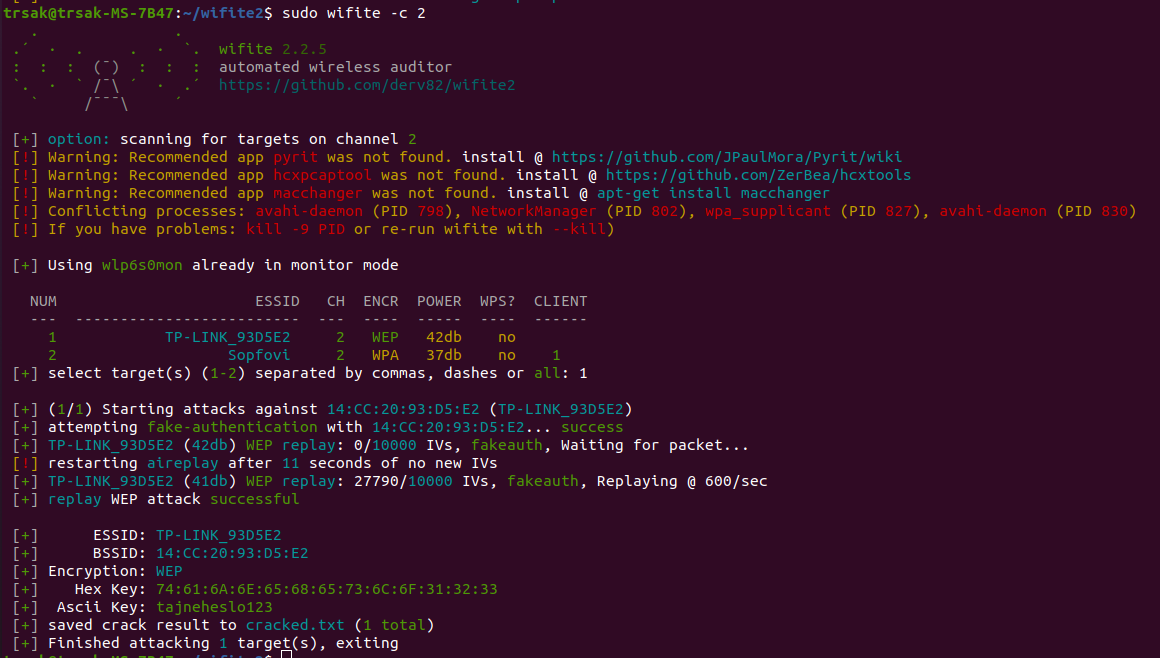
\includegraphics[width=14.7cm]{obrazky-figures/wifite.png}
  \caption{Ukázka útoku za použití Wifite2.}
  \label{img:wifite}
\end{figure}

\subsection{Cain and Abel}
Jedná se o nástroj pro Windows určený pro prolamování hesel. Podporuje prolomení spousty druhů hesel, včetně těch do Wi-Fi sítí za pomocí odposlechu paketů. Hesla následně prolamuje za pomocí metody hrubé síly, slovníkových útoků nebo s využitím kryptoanalýzy. Kryptoanalýzu provádí za pomocí tzv. duhových tabulek. Tyto tabulky obsahují seznamy již vypočítaných hodnot různých hašovacích funkcí. Nástroj nabízí opravdu velkou škálu možných útoků, především pak:
\begin{itemize}
  \item{WEP Cracking,}
  \item{ARP Spoofing,}
  \item{prolomení hashe sdílených klíčů RADIUS serveru}
\end{itemize}

\subsection{NetStumbler}
Bezplatný nástroj\footnote{Ke stažení na adrese \url{http://www.netstumbler.com/downloads/}} pro systémy Windows určený ke shromažďování informací o přístupových bodech v okolí. Používá se především v rámci wardrivingu k objevení špatně konfigurovaných přístupových bodů, na které může následně útočník provést útok. 

\subsection{coWPAtty}
Jedná se o volně dostupný nástroj\footnote{Ke stažení na adrese \url{https://github.com/joswr1ght/cowpatty}} napsaný v jazyku C určený k útokům na předsdílené klíče WPA-PSK metodou hrubé síly či slovníkovým útokem. Samotný nástroj však provádí pouze offline útok, při jeho spuštění je tedy nutné mu zaslat soubor se zachycenými pakety autentizace klienta s přístupovým bodem. 

\subsection{monkey\_jack}
Součástí programu AirJack suite, který je volně dostupný pro platformu Linux, je i nástroj monkey\_jack. Nástroj je používán pro man-in-the-middle útoky. Vše co útočník potřebuje je MAC adresa klienta, MAC adresa přístupového bodu, SSID a číslo nového kanálu. O~vše ostatní se už postará automatizovaný nástroj monkey\_jack. S nástrojem se pracuje následovně:
\begin{lstlisting}[language=bash]
./monkey_jack -b <bssid> -v <mac_klienta> -C <cislo_kanalu> [ -e <essid> ]
[ -i <nazev_rozhrani> ] [ -I <nazev_rozhrani> ]
\end{lstlisting}
Pokud tedy útočník zná všechny potřebné parametry, může snadno zahájit man-in-the-middle útok.

\subsection{Ettercap}
Ettercap\footnote{Ke stažení na adrese \url{https://www.ettercap-project.org/}} je volně dostupný program, který mimo jiné umožňuje provést takzvaný ARP spoofing, což umožní útočníkovi vytvořit podvrh ARP dotazu a vydávat se tak v~místní síti za jiného klienta. ARP je využívání pro přiřazení MAC adresy k IP adrese zařízení v~místní síti. Tabulka ARP tak obsahuje všechny známé IP adresy v~dané síti a MAC adresy k nim přiřazené. 

Pokud k nějaké IP adrese nemá ARP přiřazenou MAC adresu, pak vyšle všem zařízením v místní síti dotaz, zda daná IP adresa nepatří právě jim (viz obr. \ref{img:arp}). ARP však nenabízí žádné ověření, že odpověď přišla od validního klienta. Útočník tak může vytvořit vlastní odpověď se svojí MAC adresou, čímž dojde k otrávení mezipaměti ARP \cite{fleck2001wireless}. Všechny dotazy mířené na danou IP adresu jsou pak tedy směrovány na MAC adresu útočníka.

\subsection{Wifiphisher}
Jedním z nejpoužívanějších nástrojů pro man-in-the-middle útoky je \textbf{Wifiphisher}\footnote{Ke stažení na adrese \url{https://github.com/wifiphisher/wifiphisher}}. Jednou z funkcí tohoto nástroje je například zablokovat uživateli přístup k internetu a to až do doby, dokud uživatel nezadá heslo k Wi-Fi do podstrčeného formuláře (viz obr. \ref{img:web}). Dále umožňuje uživateli podstrčit i web s konfigurací routeru nebo v případě KARMA metody třeba přihlášení na sociální sítě. Mezi hlavní přednosti Wifiphisheru patří:

\begin{itemize}
  \item{\textbf{Výkon} -- možnost běžet hodiny na zařízeních jako Raspberry Pi a provádět všechny nejmodernější techniky k připojení do Wi-Fi sítě.}
  \item{\textbf{Flexibilita} -- spousta volitelných argumentů a dostupných šablon pro phising útoky.}
  \item{\textbf{Modulárnost} -- nástroj je možné rozšířit o jednoduché i složité pluginy psané v jazyce Python.}
  \item{\textbf{Jednoduché použití} -- zatímco zkušenější uživatelé si mohou nástroj upravit dle vlastních potřeb, nástroj může využít i méně zkušený uživatel za pomocí jednoduchého textového uživatelského prostředí.}
  \item{\textbf{Volně dostupný kód} -- volně dostupný kód pod licencí GPLv3.}
\end{itemize}

Wifiphisher se zaměřuje na získání pozice man-in-the-middle (MITM) -- jedná se o~prostředníka, který se asociuje s ostatními klienty Wi-Fi bez jejich vědomí. K dosažení tohoto cíle Wifiphisher využívá:
\begin{itemize}
  \item{\textbf{Evil Twin} -- vytvoření kopie skutečné přístupového bodu.}
  \item{\textbf{KARMA} -- vytvoření přístupového bodu, který se tváří jako veřejně dostupný.}
  \item{\textbf{Known Beacons} -- vysílání slovníku s ESSID, ke kterým se v okolí často připojovalo.}
\end{itemize}
V průběhu všech zmíněných možností také dochází k \uv{deautentizaci} nebo \uv{odloučení} paketů existujících spojení za účelem nalákání klientů na některou z výše uvedených technik.

\begin{figure}[htbp]
  \centering
  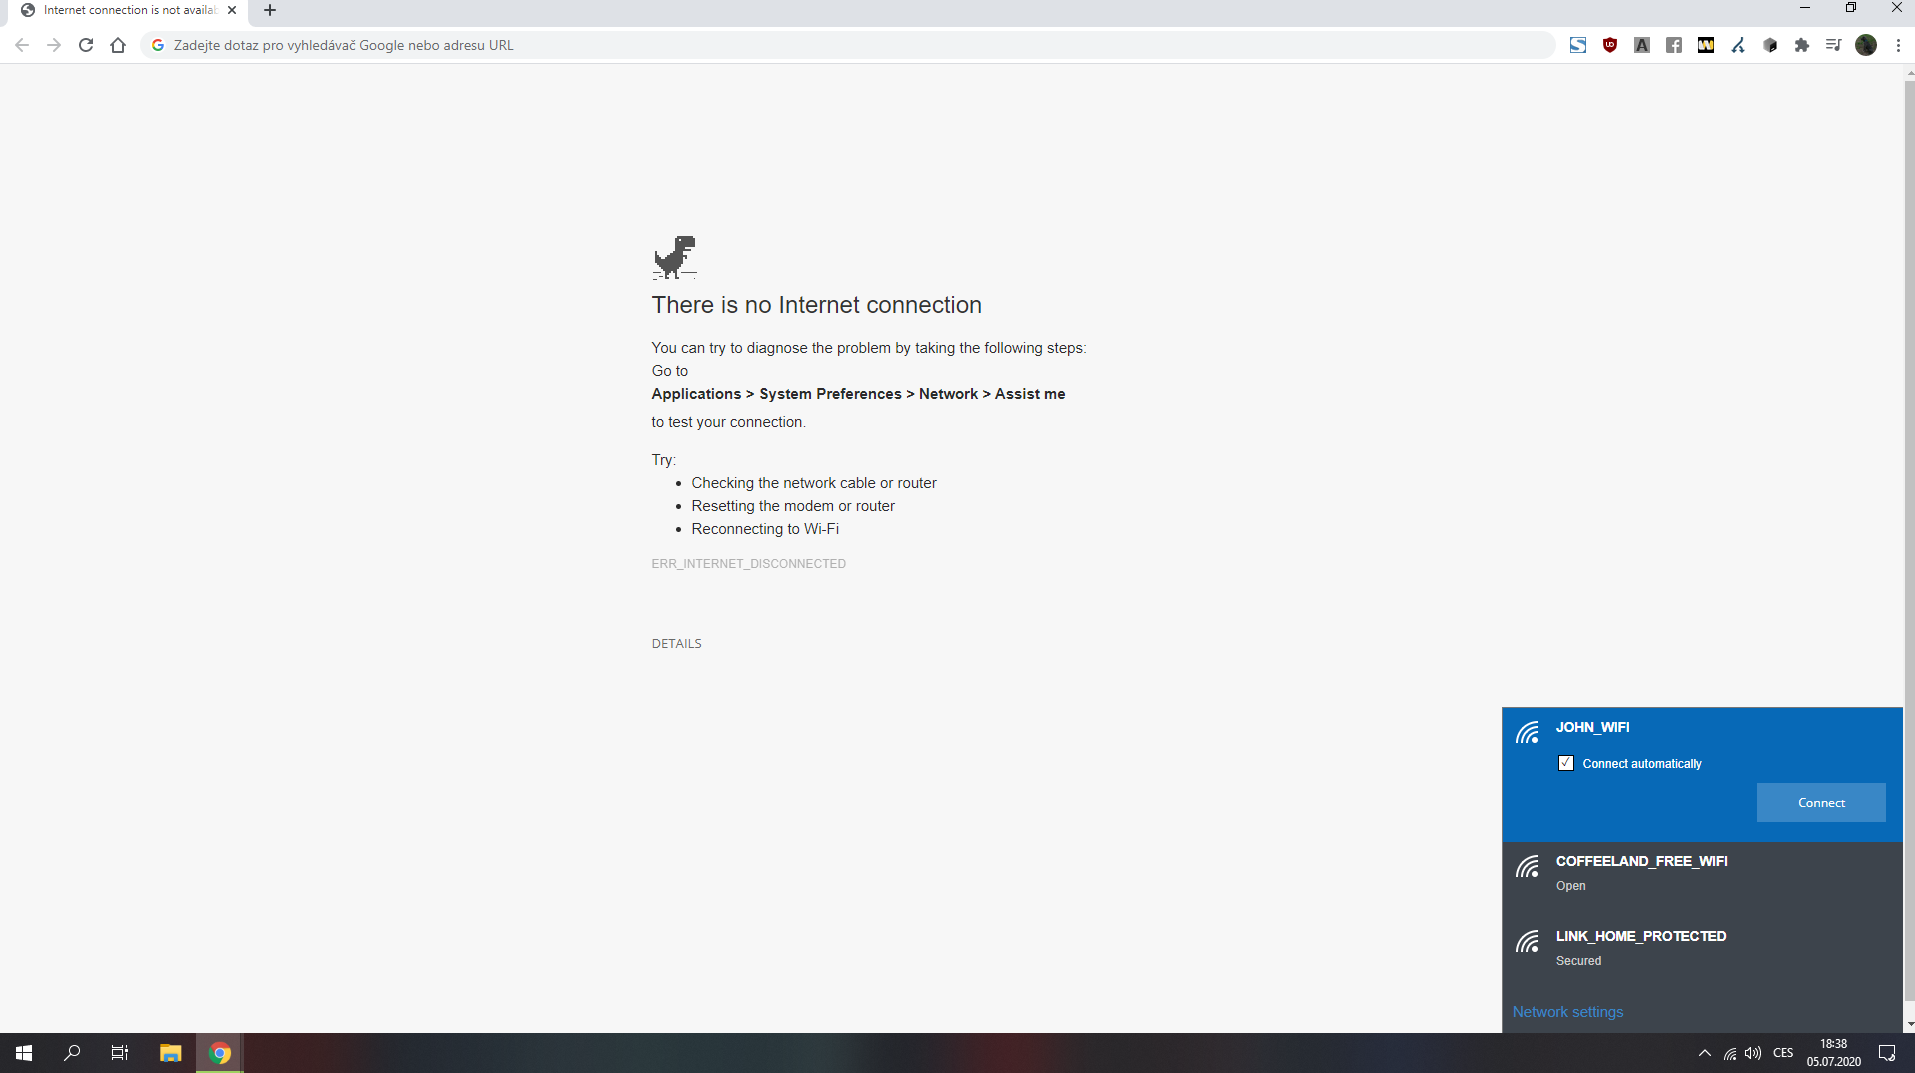
\includegraphics[width=14.7cm]{obrazky-figures/phishing.png}
  \caption{Webová stránka podstrčená uživateli za účelem získání hesla od Wi-Fi.}
  \label{img:web}
\end{figure}

\section{Testování nástrojů}
Testování nástrojů probíhalo ve vytvořené domácí síti. Spouštěny jsou z počítače s grafickou kartou MSI GeForce GTX 1080 ARMOR 8G OC, procesorem i5--8600K a síťovou kartou TP--LINK TL--WN881ND. Přístupový bod je zprovozněn na bezdrátovém routeru TL--WR841N.

\subsection{WEP Cracking}
\subsubsection*{WEP 64--bitový klíč}
Pro první testování bylo použito náhodně vygenerované heslo \texttt{G3tg3} (viz tabulka \ref{table:wep64-1}), ve druhém testu bylo použito heslo \texttt{ZW8ut} (viz tabulka \ref{table:wep64-2}). Zmíněné tabulky zobrazují přehled testovaných nástrojů, celkovou dobu, kterou trvalo prolomení hesla a počet inicializačních vektorů, které nástroj shromáždil. Doba se počítá od spuštění samotného prolamování nástrojem.

\begin{table}[htb]
\parbox{.45\linewidth}{
\centering
\begin{tabular}{|c|c|c|}
\hline
\textbf{Nástroj} & \textbf{Doba} & \textbf{Počet IV} \\ \hline
Aircrack         & 1m 37s                & 27320                   \\ \hline
Airgeddon        & 2m 18s                & 48224                   \\ \hline
Besside-ng       & 2m 14s                & 46412                   \\ \hline
Wifite2          & 1m 42s                & 34955                   \\ \hline
LAZY script      & 4m 08s                & 67247                   \\ \hline
\end{tabular}
\caption{Prolamování 64--bitového WEP -- heslo \texttt{G3tg3}.}
\label{table:wep64-1}
}
\hfill
\parbox{.45\linewidth}{
\centering
\begin{tabular}{|c|c|c|}
\hline
\textbf{Nástroj} & \textbf{Doba} & \textbf{Počet IV} \\ \hline
Aircrack         & 1m 24s                & 24478                   \\ \hline
Airgeddon        & 2m 01s                & 43544                   \\ \hline
Besside-ng       & 2m 18s                & 47252                   \\ \hline
Wifite2          & 1m 44s                & 33429                   \\ \hline
LAZY script      & 3m 58s                & 62470                   \\ \hline
\end{tabular}
\caption{Prolamování 64--bitového WEP -- heslo \texttt{ZW8ut}.}
\label{table:wep64-2}
}
\end{table}

\subsubsection*{WEP 128--bitový klíč}
V prvním testování bylo použito náhodně vygenerované heslo \texttt{EX4LtrU9nEuD6} (viz tabulka \ref{table:wep128-1}) a ve druhém heslo \texttt{Ay6PWddD9kHEq} (viz tabulka \ref{table:wep128-2}). Tabulky zobrazují přehled testovaných nástrojů. Doba se počítá od spuštění samotného prolamování nástrojem.

\begin{table}[htb]
\parbox{.45\linewidth}{
\centering
\begin{tabular}{|c|c|c|}
\hline
\textbf{Nástroj} & \textbf{Doba} & \textbf{Počet IV} \\ \hline
Aircrack         & 2m 34s                & 45610                   \\ \hline
Airgeddon        & 3m 24s                & 88224                   \\ \hline
Besside-ng       & 4m 21s                & 110176                  \\ \hline
Wifite2          & 2m 56s                & 62955                   \\ \hline
LAZY script      & 7m 46s                & 184647                  \\ \hline
\end{tabular}
\caption{Prolamování 128--bitového WEP -- heslo \texttt{EX4LtrU9nEuD6}.}
\label{table:wep128-1}
}
\hfill
\parbox{.45\linewidth}{
\centering
\begin{tabular}{|c|c|c|}
\hline
\textbf{Nástroj} & \textbf{Doba} & \textbf{Počet IV} \\ \hline
Aircrack         & 2m 52s                & 51477                   \\ \hline
Airgeddon        & 3m 43s                & 92784                   \\ \hline
Besside-ng       & 3m 58s                & 93214                  \\ \hline
Wifite2          & 3m 03s                & 64529                   \\ \hline
LAZY script      & 7m 12s                & 163437                  \\ \hline
\end{tabular}
\caption{Prolamování 128--bitového WEP -- heslo \texttt{Ay6PWddD9kHEq}.}
\label{table:wep128-2}
}
\end{table}

\subsubsection*{Vyhodnocení}
Nejlépe dopadl nástroj Aircrack, který využívá i většina automatizovaných nástrojů. Z~automatizovaných nástrojů vyšel nejlépe Wifite2. Graf \ref{img:wep-vysledky} zobrazuje celkovou dobu nástroje pro všechny testy v sekundách, menší hodnota značí lepší výsledek.

\subsection{WPA/WPA2 Offline cracking}
Pro testování offline prolamování hesel WPA a WPA2 byla zvolena hesla \texttt{secretpassword} a \texttt{2153*bulldogge\#841}. Následně byl zahájen slovníkový útok se všemi nástroji, které se použily i při WEP crackingu. První zmíněné heslo se ve slovníku hesel nacházelo na řádku 40~498 a druhé heslo na řádku 35~025~995.

Všechny testované nástroje používají stejné metody pro offline cracking a tak se výsledná doba prolomení hesla lišila pouze v řádech sekund, maximálně několika minut. Průměrná rychlost prolamování byla 14~127 hesel za sekundu. První heslo se tak podařilo prolomit za necelé tři sekundy, zatímco druhé heslo zabralo zhruba 42 minut.

\subsection{Celkové vyhodnocení}
Cílem bylo najít nejlepší automatizovaný nástroj pro prolamování zabezpečení Wi-Fi sítí. Nejlépe v testech skončil nástroj Wifite2, který se po zadání argumentů v podobě cílového BSSID a síťového rozhraní o vše automaticky postará -- zvolí nejlepší metodu útoku a~následně se pokusí heslo prolomit. 

\begin{figure}[htbp]
  \centering
  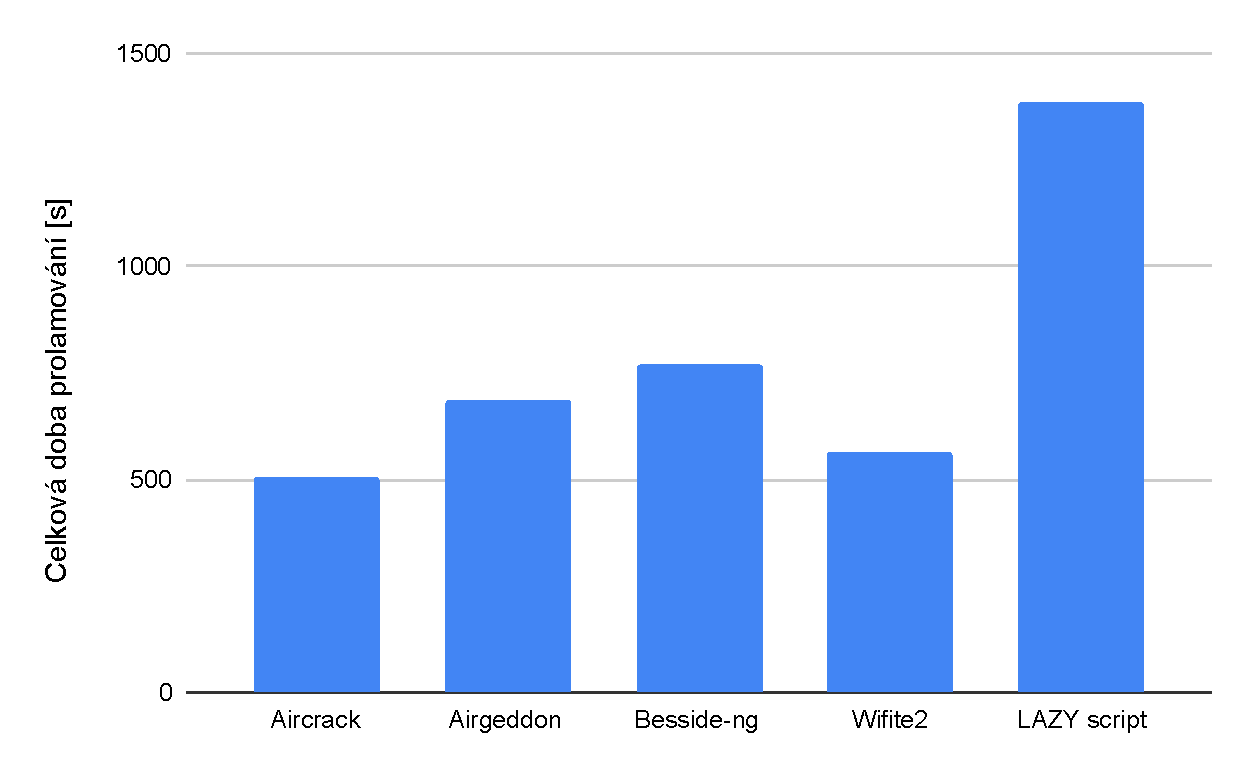
\includegraphics[width=15cm]{obrazky-figures/porovnani-wep.pdf}
  \caption{Graf celkové doby prolamování hesel do Wi-Fi sítí jednotlivých nástrojů pro všechny provedené testy prolamování WEP. Menší hodnota značí lepší výsledek.}
  \label{img:wep-vysledky}
\end{figure}

\chapter{Návrh nástroje pro odposlech komunikace}
\label{navrh}
Tato kapitola popisuje návrh nástroje pro odposlech komunikace mezi klientem a přístupovým bodem. Cílem je vytvořit nástroj, který bude zachytávat pakety mezi určitým klientem a přístupovým bodem. Tyto pakety následně bude dešifrovat za pomocí hesla získaného nástrojem Wifite2. V případě samostatného zařízení pak bude dešifrované pakety ukládat do samostatného souboru, v případě integrace do sondy pak bude spolupracovat se sondou.

\section{Knihovny pro zachycení síťového provozu}
Pro zachycení síťového provozu existuje řada knihoven. Následuje přehled dvou z nich a~jejich následné porovnání.

\subsection{Libpcap}
Jedná se o voldě dostupnou knihovnu\footnote{Libpcap je dostupný na adrese \url{https://www.tcpdump.org/}} pro programy psané v jazyce C/C++. Nabízí velkou škálu možností pro zachytávání síťového provozu a následné práce se zachycenými pakety. Tuto knihovnu využívají programy jako tcpdump či WireShark. Výhodou této knihovny je především to, že pokud operační systém nabízí možnost pracovat s paketovým filtrem kernelu, pak knihovna dokáže filtrovat data přímo v rámci kernelu (jádro operačního systému). 

\subsection{Libtins}
Libtins je volně dostupná\footnote{Libtins je dostupný na adrese \url{http://libtins.github.io/}} multiplatformní knihovna psaná v jazyce C++. Nabízí nástroje pro odposlech síťového provozu a sestavování paketů. Knihovna vznikla s cílem umožnit vývojářům snadnou a přes to efektivní cestu jak vytvořit nástroje pracující s pakety v síti. Celá knihovna byla navržena tak, aby i přes její snadné použití byla zachována efektivita. Knihovna nabízí především:
\begin{itemize}
  \item{sestavování paketů,}
  \item{odposlech paketů a jejich automatické parsování,}
  \item{zápis a čtení pcap souborů,}
  \item{dešifrování datových rámců WEP a WPA/WPA2 (TKIP A CCMP).}
\end{itemize}

\subsection{Porovnání knihoven}
Největším problémem knihovny Libtins je, že neumožňuje neblokující odposlech paketů za použití pouze jednoho vlákna, což implementace do sondy vyžaduje. Implementace odposlechu paketů s knihovnou Libtins je však značně snadnější, jelikož parsování jednotlivých paketů knihovna provádí sama.

Co se týče rychlosti jednotlivých knihoven, knihovna libpcap vychází ze všech testů jako rychlejší. Při zátěžovém testu, ve kterém bylo parsováno 500~000 DNS paketů ze souboru (viz obr. \ref{img:knihovny}) zvládla knihovna libpcap pakety zpracovávat rychlostí 13~888~888 paketů za sekundu, zatímco knihovna libtins zvládla 1~278~772 paketů za sekundu\footnote{Údaje dostupné z \url{http://libtins.github.io/benchmark/}}.
\begin{figure}[htbp]
  \centering
  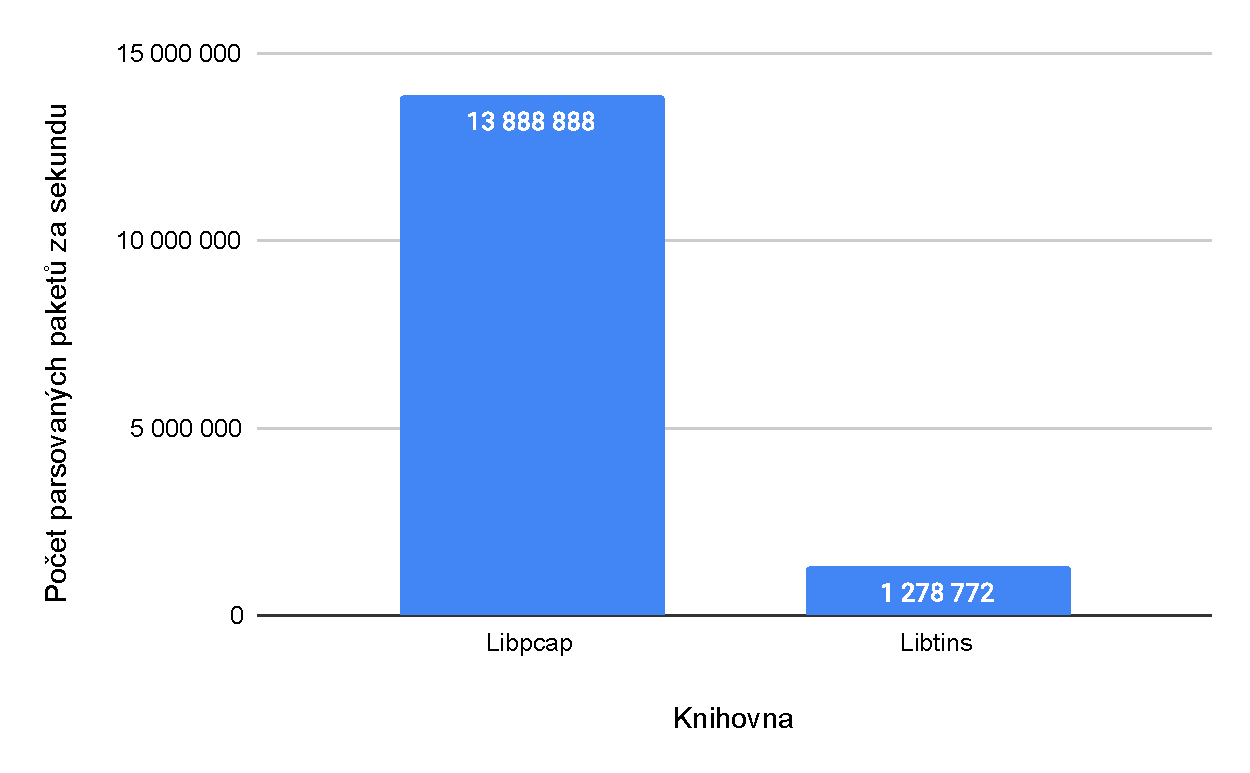
\includegraphics[width=15cm]{obrazky-figures/knihovny.pdf}
  \caption{Počet paketů parsovaných za sekundu při parsování 500~000 DNS paketů ze souboru za použití knihoven Libpcap a Libtins.}
  \label{img:knihovny} 
\end{figure}

Odposlech paketů pro implementaci nástroje do sondy bude proveden jen za pomocí knihovny libpcap, aby došlo k zachování jedno-vláknového a neblokujícího zpracování paketů. Implementace pro samostatné zařízení pak bude umožňovat použití obou knihoven, mezi kterými si může uživatel vybírat za pomocí přepínače.

\section{Zachycení komunikace mezi klientem a přístupovým bodem}
Síťové karty obvykle nabízejí dva různé speciální režimy:
\begin{enumerate}
  \item{\textbf{Promiskuitní režim} - tento režim umožňuje zachytávat veškeré pakety v rámci sítě, do které je klient připojen. Oproti běžnému režimu tak síťová karta zachytává i pakety, které jsou určeny pro jiného příjemce v síti.}
  \item{\textbf{Monitorovací režim} - nevyžaduje asociaci s přístupovým bodem a umožňuje tak zachytávat veškerou komunikaci libovolného klienta a přístupového bodu v dosahu.}
\end{enumerate}
Pro účely odposlouchávání tak program přepne síťovou kartu do monitorovacího režimu. Z toho důvodu je výsledný program nutné spouštět se speciálním oprávněním. Za pomocí tohoto režimu pak můžeme komunikaci mezi klient se zadanou MAC adresou a~přístupovým bodem se zadaným BSSID odposlouchávat za pomocí aplikování filtru:
\begin{lstlisting}[language=bash]
wlan addr3 BSSID and (wlan addr1 MAC or wlan addr2 MAC)
\end{lstlisting}
V případě nutnosti zachytit i broadcast vysílání přístupového bodu by filtr vypadal následovně:
\begin{lstlisting}[language=bash]
wlan addr3 BSSID and (wlan addr1 MAC or wlan addr2 MAC or wlan addr1 ff:ff:ff:ff:ff:ff)
\end{lstlisting}

Některé procesy systému provádí kontrolu připojení a mnohdy v moment, kdy zjistí, že kvůli monitorovacímu režimu není dostupné připojení, navrátí síťovou kartu opět do běžného režimu. V takovém případě je nutné využít nástroje airmon-ng a před spuštěním programu vynutit ukončení těchto procesů příkazem:
\begin{lstlisting}[language=bash]
airmon-ng check kill
\end{lstlisting}

\section{Hlavička RadioTap}
Nedílnou součástí práce s pakety v rámci Wi-Fi síti jsou hlavičky RadioTap. Jedná se o mechanismus používaný k přidání dodatečných informací o jednotlivých rámcích. Obrázek~\ref{img:radiotap} zobrazuje strukturu hlavičky RadioTap programem Wireshark.
\begin{figure}[htbp]
  \centering
  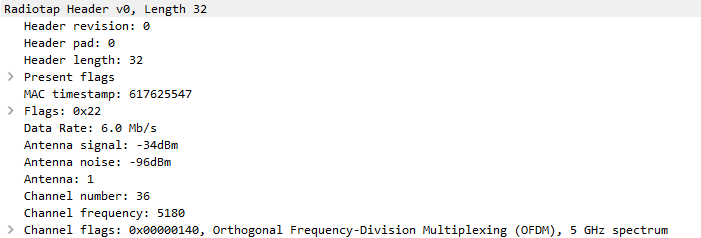
\includegraphics[width=14cm]{obrazky-figures/radiotap.png}
  \caption{Struktura hlavičky RadioTap vyobrazená programem Wireshark.}
  \label{img:radiotap}
\end{figure}

Hlavičku přidává síťový adaptér nebo jeho ovladač, který daný paket zachytil. Drtivá většina moderní síťových karet hlavičky RadioTap přidává, především u starších karet však jejich přítomnost není zaručena. Z hlavičky můžeme vyčíst zajímavé informace, jako jsou například:
\begin{itemize}
  \item{síla signálu,}
  \item{číslo a frekvence použitého kanálu,}
  \item{informace o použité anténě,}
  \item{příznaky s informacemi o fragmentaci a struktuře paketu.}
\end{itemize}

\section{Detekce použitého protokolu pro šifrování}
Aby program věděl, zda a jakým způsobem je nutné data dešifrovat, musí provést detekci použitého protokolu pro šifrování. Detekovat šifrování může v rámci Beacon rámce. Beacon rámec obsahuje informace o způsobilosti (tzv. Capability Information) -- příznak Privacy značí, zda-li používá přístupový bod nějaké šifrování (viz obr. \ref{img:Beacon-capability}). 
\begin{figure}[htbp]
  \centering
  \includegraphics[width=14cm]{obrazky-figures/Beacon-capability.png}
  \caption{Informace o způsobilosti sítě v rámci Beacon rámce. Převzato z \cite{gast2017802}.}
  \label{img:Beacon-capability}
\end{figure}

Pokud síť používá nějaký protokol pro šifrování (tedy příznak Privacy má hodnotu~1), pak je nutné detekovat konkrétní použité šifrování. Informaci o konkrétním šifrování lze nalézt v rámci části Robust Security Network (RSN). Pokud přijatý paket RSN neobsahuje, pak síť využívá protokolu WEP. Obrázek \ref{img:rsn} zobrazuje strukturu RSN.
\begin{figure}[htbp]
  \centering
  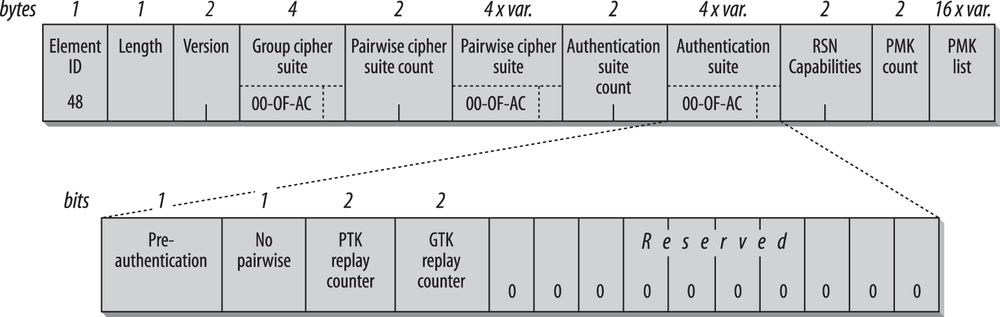
\includegraphics[width=14cm]{obrazky-figures/rsn.png}
  \caption{Struktura Robust Security Network (RSN) obsaženého v Beacon rámci. Převzato z \cite{gast2017802}.}
  \label{img:rsn}
\end{figure}

Za pomocí části skupinové šifry (Group cipher suite) v RSN je možné určit konkrétní použité šifrování. Selektor šifry má délku čtyři bajty. Skládá se ze dvou částí, první část je tzv. OUI pro dodavatele a druhá část značí již konkrétní šifru. Protokol IEEE 802.11i používá OUI \texttt{00-0F-AC}. Tabulka \ref{table:gcs} zobrazuje standardizované sady šifer. Díky tomu tedy můžeme detekovat konkrétní šifrování, které využívá přístupový bod pro přenos datových rámců. V případě použití staršího WPA však RSN v rámci nenalezneme. Místo něho nalezneme v~rámci tzv. specifický vendor WPA prvek s identifikačním číslem 221. OUI je v~tomto případě \texttt{00-50-F2}, tabulka \ref{table:wpa-oui} zobrazuje možnost detekci šifrování na základě tohoto prvku.

\begin{table}[htb]
\centering
\begin{tabular}{|c|c|c|}
\hline
\textbf{OUI} & \textbf{Typ šifry} & \textbf{Definice} \\ \hline
00-0F-AC     & 1                  & WEP-40            \\ \hline
00-0F-AC     & 2                  & TKIP              \\ \hline
00-0F-AC     & 3                  & Rezervováno       \\ \hline
00-0F-AC     & 4                  & CCMP              \\ \hline
00-0F-AC     & 5                  & WEP-104           \\ \hline
00-0F-AC     & 6                  & BIP-CMAC-128           \\ \hline
00-0F-AC     & 8                  & GCMP-128           \\ \hline
00-0F-AC     & 9                  & GCMP-256           \\ \hline
00-0F-AC     & 10                  & CCMP-256           \\ \hline
00-0F-AC     & 11                  & BIP-GMAC-128           \\ \hline
00-0F-AC     & 12                  & BIP-GMAC-256           \\ \hline
00-0F-AC     & 13                  & BIP-CMAC-256           \\ \hline
\end{tabular}
\caption{Detekce použitého šifrování na základě hodnoty GCS skupinové šifry v RSN. Převzato z \cite{gast2017802}.}
\label{table:gcs}
\end{table}

\begin{table}[htb]
\centering
\begin{tabular}{|c|c|c|}
\hline
\textbf{OUI} & \textbf{Typ šifry} & \textbf{Definice} \\ \hline
00-50-F2     & 0                  & Hodnota v GCS           \\ \hline
00-50-F2     & 1                  & WEP-40              \\ \hline
00-50-F2     & 2                  & TKIP       \\ \hline
00-50-F2     & 3                  & Rezervováno              \\ \hline
00-50-F2     & 4                  & Rezervováno           \\ \hline
00-50-F2     & 5                  & WEP-104           \\ \hline
\end{tabular}
\caption{Detekce použitého šifrování na základě hodnoty informačního elementu WPA.}
\label{table:wpa-oui}
\end{table}

\section{Problémy spojené s odposloucháváním}
Samotné odposlouchávání může být mnohdy velmi problematické. Prvním problémem je detekovatelnost odposlouchávání. Pokud není provedena deautentizace klienta, pak celý odposlech probíhá pasivně a není tedy detekovatelný. Deautentizace klienta však celý proces značně urychluje, jelikož není nutné čekat na znovupřipojení klienta do sítě. Dalším problémem je nutnost spouštět nástroj se speciálním oprávněním, aby bylo možné síťové rozhraní pomocí programu přepnout do monitorovacího režimu.

Největším problémem je však nutnost mít kompatibilní a správně nastavený hardware. Zařízení pro odposlouchávání může z důvodu špatné kompatibility odposlouchávat provoz pouze v omezené míře, nebo dokonce vůbec. Mezi hlavní problémy při špatné kompatibilitě se řadí: 
\begin{itemize}
  \item{\textbf{Rozdílná frekvence} -- 2.4 nebo 5 GHz.}
  \item{\textbf{Rozdílná šířka pásma} -- 20/40/80 MHz.}
  \item{\textbf{Rozdílný prostorový tok} -- tzv. Spatial stream, dostupné jsou čtyři druhy.}
  \item{\textbf{Rozdílný guard interval} -- může být dlouhý nebo krátký, zabezpečuje mezery mezi jednotlivými pakety.}
\end{itemize}


\chapter{Implementace nástroje}
\label{implementace}
Tato kapitola pojednává o implementaci nástroje pro odposlech komunikace mezi klientem a přístupovým bodem. Implementace se dále dělí na dvě části -- implementace nástroje do sondy a do samostatného zařízení. Obě části implementace jsou napsány v jazyce C++. Výsledkem implementace jsou konzolové programy pro platformu Linux.

\section{Architektura programu}
Obrázek \ref{img:sniffer-classes} popisuje diagram hlavních tříd programu. Architektura programu je navržena tak, aby bylo možné později přidat další případné knihovny na odposlouchávání síťového provozu.

\begin{figure}[htbp]
  \centering
  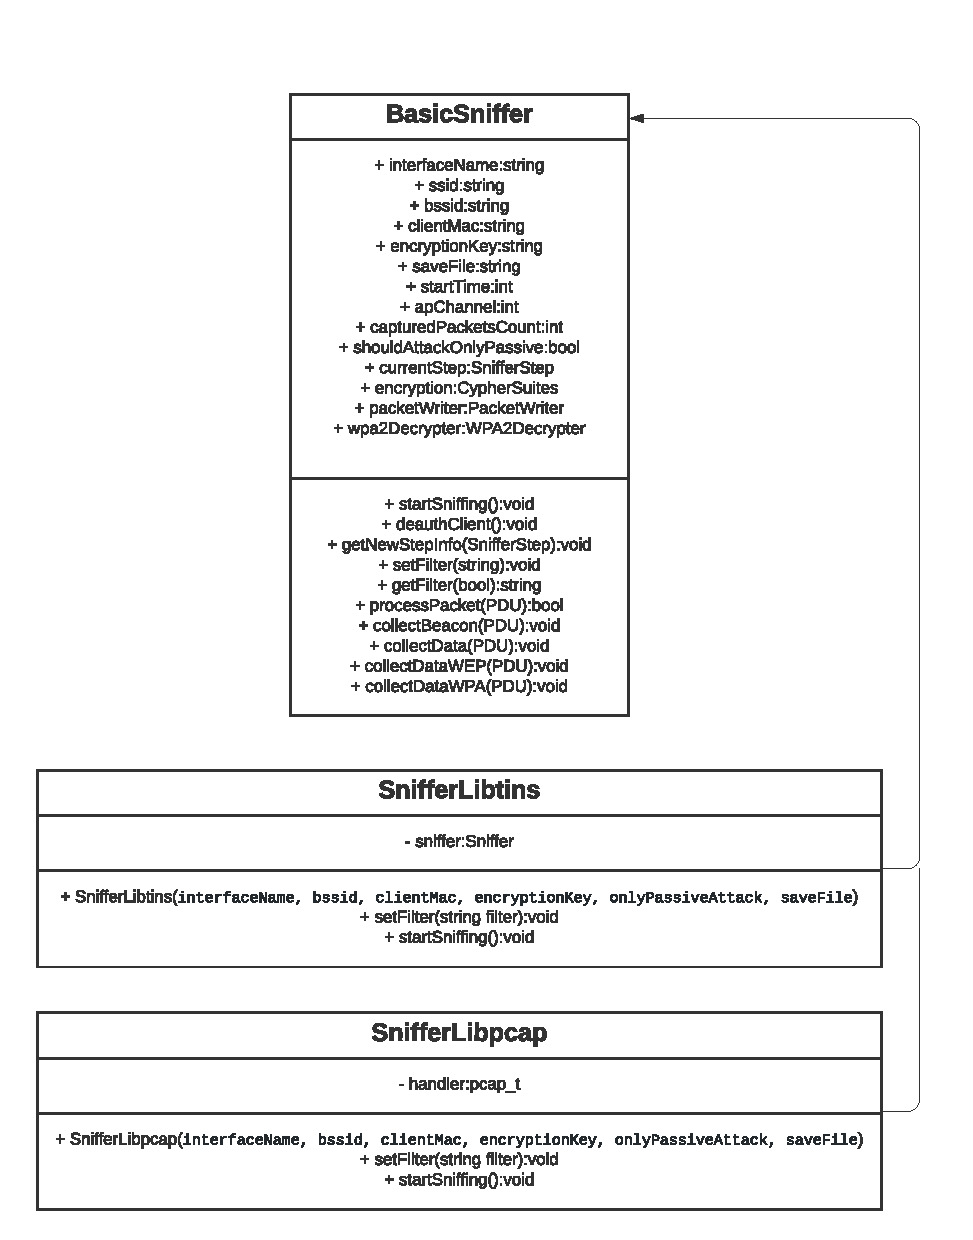
\includegraphics[width=14.7cm]{obrazky-figures/Sniffer.pdf}
  \caption{Diagram tříd nástroje pro odposlouchávání komunikace mezi klientem a přístupovým bodem.}
  \label{img:sniffer-classes}
\end{figure}

\subsection{Abstraktní třída BasicSniffer}
Abstraktní třída BasicSniffer zastřešuje hlavní metody a jednotlivé kroky při odposlechu sítě. Celý nástroj postupně prochází těmito kroky: 
\begin{enumerate}
  \item{\textbf{Spuštění odposlechu} - dojde k nastavení síťového rozhraní do monitorovacího modu. Následně je nastaven filtr, který zajišťuje zachytávání komunikace pouze mezi zvoleným klientem a přístupovým bodem.}
  \item{\textbf{Zachycení Beacon rámce} - dalším krokem je zachycení Beacon rámce, ze kterého získáme další údaje o síti jako SSID, kanál a další. Z Beacon rámce také nástroj detekuje šifrování použité přístupovým bodem.}
  \item{\textbf{Deautentizace klienta a zachycení 4-fázového autentizačního handshake} - provede se jen v případě, pokud přístupový bod používá šifrování TKIP nebo CCMP. Deautentizace je provedena jen v případě, kdy je povoleno aktivní sondování a není přepínačem vynucen pouze pasivní útok. V opačném případě nástroj čeká, dokud autentizaci nezachytí.}
  \item{\textbf{Zachytávání paketů} - následně dochází k zachytávání paketů. Pokud bylo detekováno nějaké šifrování, jsou jednotlivé pakety před zpracováním dešifrovány za pomocí hesla na vstupu programu.}
\end{enumerate}

Třída k parsování paketů a jejich případnému dešifrování využívá knihovny libtins. Z této třídy pak dědí třídy SnifferLibtins a SnifferLibpcap.

\subsection{Třídy SnifferLibpcap a SnifferLibtins}
Tyto třídy dědí ze třídy BasicSniffer. Úkolem těchto tříd je především implementace metody \textit{startSniffing} v závislosti na zvolené knihovně. Obě třídy zajišťují postupně následující úkony:
\begin{enumerate}
  \item{nastavení síťového rozhraní do monitorovacího režimu,}
  \item{nastavení časového limitu,}
  \item{nastavení neblokujícího čtení (pouze u libpcap),}
  \item{nastavení filtru,}
  \item{spuštění odposlechu.}
\end{enumerate}

\section{Deautentizace klienta}
Pro provedení deautentizace klienta je nutné sestrojit a zaslat deautentizační rámec. Nejprve je nutné sestrojit RadioTap hlavičku se shodným kanálem, na kterém vysílá přístupový bod. Následně je přidán deautentizační rámec, kde je BSSID přístupového bodu označen jako zdroj a MAC adresa klienta jako cíl. Jelikož může docházet k rušení, těchto paketů je sestaveno a odesláno celkem deset. Obrázek \ref{img:deauth-wireshark} vyobrazuje sestavený deautentizační rámec programem Wireshark.
\begin{figure}[htbp]
  \centering
  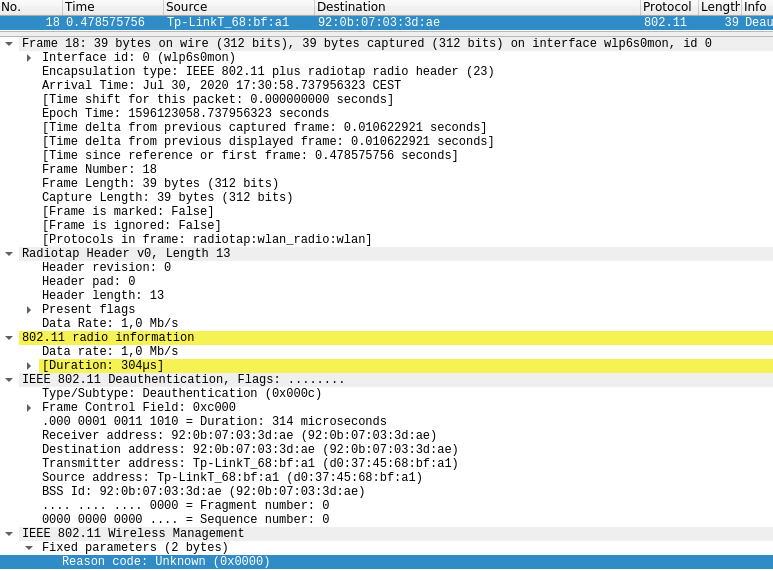
\includegraphics[width=14.9cm]{obrazky-figures/deauth-wireshark.png}
  \caption{Sestavený deautentizační rámec zobrazený programem Wireshark.}
  \label{img:deauth-wireshark}
\end{figure} 

\section{Implementace do samostatného zařízení}
V případě implementace do samostatného zařízení není nutné udržovat odposlech jako neblokující a je tak možné využít knihovnu libtins i libpcap. Činnost programu lze ovlivnit použitím následujících parametrů: 
\begin{itemize}
  \item{\textbf{-i} -- povinný parametr, název rozhraní které bude přepnuto do monitorovacího režimu a použito k odposlechu.}
  \item{\textbf{-b} -- povinný parametr, BSSID přístupového bodu.}
  \item{\textbf{-m} -- povinný parametr, MAC Adresa klienta.}
  \item{\textbf{-k} -- klíč použitý k dešifrování WEP/WPA/WPA2.}
  \item{\textbf{-f} -- cesta k .pcap souboru, do kterého budou uloženy pakety získané při odposlechu. Pokud není zadáno, data jsou uložena do souboru sniffing.pcap do adresáře, ve kterém byl program spuštěn.}
  \item{\textbf{-p} -- přepínač, který určuje, že celý odposlech bude proveden pasivně (nebude tedy provedena deautentizace klienta).}
  \item{\textbf{-l} -- vynucení použití knihovny libpcap pro odposlech.}
  \item{\textbf{-t} -- vynucení použití knihovny libtins pro odposlech.}
\end{itemize}

Po spuštění programu začne odposlech komunikace mezi zvoleným klientem a přístupovým bodem. Pokud dojde k detekování šifrování pomocí WPA nebo WPA2, program musí pro dešifrování obsahu datových rámců nejprve provést zachycení 4-fázové autentizace. Pokud není vynucen pasivní útok přepínačem \textbf{-p}, pak je provedena deautentizace klienta a~při následném znovupřipojení klienta k přístupovému bodu dojde ke zachycení potřebných paketů. Program běží a odposlouchává komunikaci až do momentu, kdy obdrží signál pro přerušení (lze vyvolat za pomocí klávesové zkratky CTRL+C). Výsledkem je soubor obsahující všechny zachycené a dešifrované pakety. Obsah souboru lze zobrazit například programem Wireshark či tcpdump.

\subsection{Testování}
Program byl testován na několika zařízení a to pro odposlech komunikace šifrované za pomocí WEP, TKIP a CCMP. Výstup programu při použití šifrování CCMP:
\begin{lstlisting}[language=bash]
sudo ./sniffer -i wlp6s0 -b "14:CC:20:93:D5:E2" -m "60:ab:67:e3:3b:9e" -k tajneheslo
Using libtins library for sniffing.
Interface wlp6s0 was set to monitor mode.
 
 
Collecting Beacon frame to gather info...
Found Beacon frame!
SSID: TP-LINK_93D5E2
Channel: 2
AP is using some sort of encryption, trying to detect...
Detected encryption: CCMP
 
We have to collect 4-way auth handshake...
Building deauthentication packets...
Sending deauthentication packet (10/10).
All deauthentication packets sent!
 
Capturing 4-way auth handshake...
 
Managed to decrypt packet data!
Captured 92 packets in 15 seconds.
Exiting...
\end{lstlisting}

Obrázek \ref{img:sniffer-wireshark} zobrazuje analýzu výsledného pcap souboru programem Wireshark. Díky nástroji se podařilo odposlechnout data šifrovaná za pomocí CCMP a následně tyto data dešifrovat a analyzovat. Z analýzy je možné například zjistit, že klient přistupoval na webovou stránku přes nezabezpečený HTTP protokol.
\begin{figure}[htbp]
  \centering
  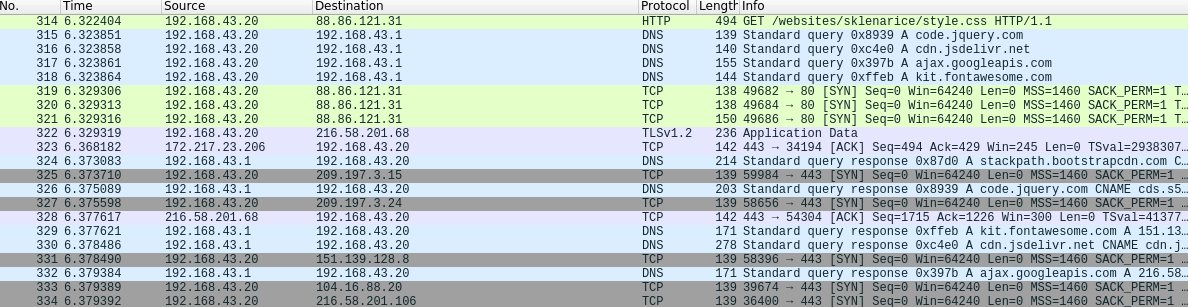
\includegraphics[width=14.9cm]{obrazky-figures/sniffer-wireshark.png}
  \caption{Analýza výstupního pcap souboru z odposlechu provedená programem Wireshark.}
  \label{img:sniffer-wireshark}
\end{figure}

\section{Implementace do sondy}
Pro implementaci nástroje do sondy bylo nutné se nejprve seznámit s existující implementací sondy a provázat s ní vytvořený nástroj. Implementace pro sondu, z důvodu aby nedocházelo k jejímu zpomalení, využívá neblokující odposlech na jednom vlákně, proto je zde použita pouze knihovna Libpcap. Program může být spuštěn s následujícími parametry:
\begin{itemize}
  \item{\textbf{-n} -- povinný parametr, název rozhraní které bude přepnuto do monitorovacího režimu a použito k odposlechu.}
  \item{\textbf{-b} -- povinný parametr, BSSID přístupového bodu.}
  \item{\textbf{-c} -- povinný parametr, MAC Adresa klienta.}
  \item{\textbf{-k} -- klíč použitý k dešifrování WEP/WPA/WPA2.}
  \item{\textbf{-A} -- umožňuje provést aktivní útok (deautentizací klienta).}
  \item{\textbf{-L} -- IP adresa sondy.}
  \item{\textbf{-P} -- port sondy.}
  \item{\textbf{-I} -- identifikátor sondy.}
\end{itemize}
Dále obsahuje parametry pro filtrování provozu, všechny parametry je možné zobrazit v~rámci nápovědy (\textbf{-h}).

Po spuštění programu dojde k inicializaci exportéru a parseru pro protokoly aplikační vrstvy. Následně program postupuje stejně, jako verze pro samostatná zařízení. Nejprve shromáždí Beacon rámec, ze kterého zjistí potřebné informace. V závislosti na detekovaném šifrování pak provede další operace. V moment, kdy dojde k úspěšnému dešifrování, jsou dešifrované rámce vraceny do hlavní smyčky programu. 
Problémem je, že sonda je implementována pro práci s Ethernetovými pakety, nikoliv pro pakety IEEE 802.11. Je tedy nutné pakety ořezat až po IP hlavičku a následně ji spojit se sestrojenou Ethernetovou hlavičkou. Takto sestavené pakety jsou pak předávány sondě dále ke zpracování. Obrázek~\ref{img:diagram-sonda} zobrazuje postupnou práci s přijatým paketem.
\begin{figure}[htbp]
  \centering
  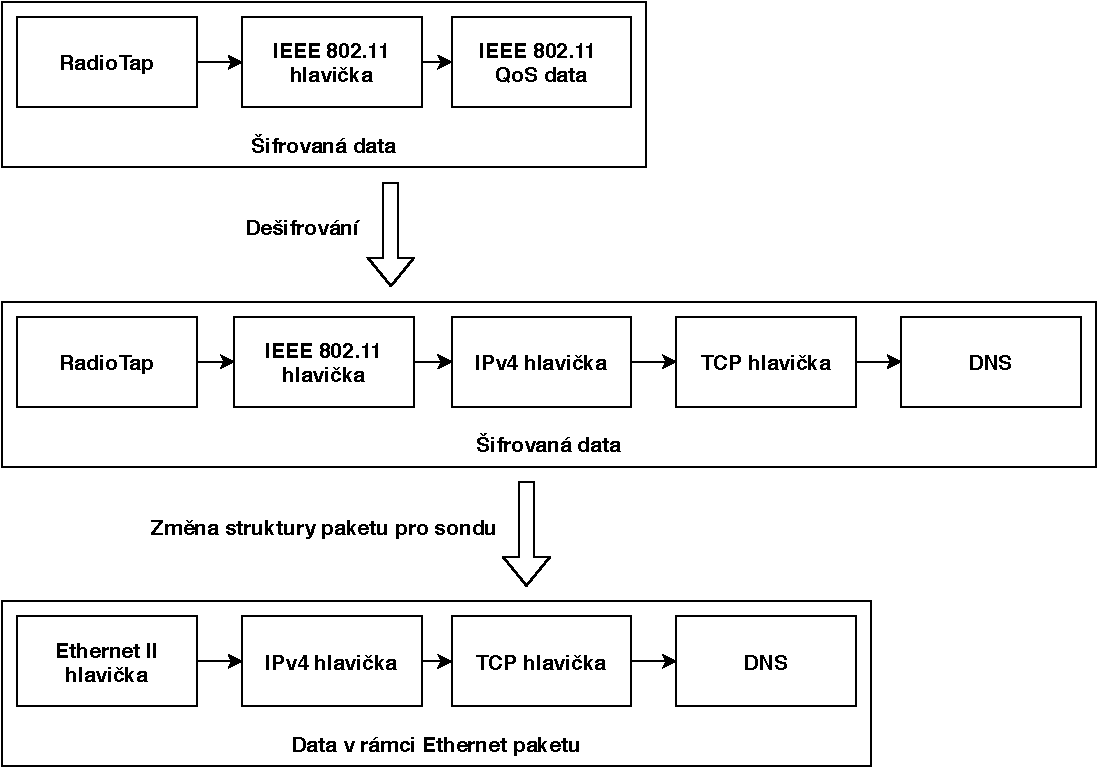
\includegraphics[width=14.9cm]{obrazky-figures/diagram-sonda.pdf}
  \caption{Ukázka postupné práce se zachyceným paketem v rámci předání paketu do sondy.}
  \label{img:diagram-sonda}
\end{figure}

\chapter{Závěr}
\label{zaver}
Cílem této bakalářské práce bylo prostudovat problematiku zabezpečení Wi-Fi sítí, porovnat nástroje používané pro útoky na Wi-Fi sítě a následně nejlepší nástroj integrovat s~vytvořeným programem pro odposlouchávání komunikace do samostatného zařízení a sondy vyvíjené na FIT VUT. 

Prvním krokem tedy bylo prostudovat strukturu Wi-Fi sítí a možnosti jejich zabezpečení. To vyžadovalo seznámení se s jednotlivými protokoly a prostudování jejich struktury a funkčnosti. Dalším krokem bylo analyzování známých druhů a typů útoků na Wi-Fi sítě využívajících chyb ve standardech IEEE 802.11. Jelikož se chyby v zabezpečení Wi-Fi sítí mnohdy netýkají jenom standardů, ale i konkrétních zařízení, tak se práce zabývá i~nejpoužívanějšími zařízeními v České republice, které obsahují kritické chyby. V další části bylo porovnáno několik existujících nástrojů pro útoky na Wi-Fi sítě. Nástroje sloužící pro prolomení WEP, WPA a WPA2 byly následně testovány a z automatizovaných nástrojů vyšel nejlépe nástroj Wifite2. Jelikož tento nástroj po instalaci dokáže plně automatizovaně provést útok na prolomení hesla do Wi-Fi sítě, tak byl následně implementován program, který za pomocí získaného hesla odposlouchává komunikaci mezi klientem a přístupovým bodem. Tento nástroj se podařilo implementovat ve dvou verzích -- pro samostatná zařízení a jako modul pro sondu vyvíjenou na FIT VUT. Vytvořený nástroj byl spolu s nástrojem Wifite2 testován pro odposlech komunikace šifrované za pomocí WEP využívajícího 40 a~104--bitového klíče. Dále na protokolu WPA využívajícího TKIP a WPA2 využívající šifrování CCMP. V případě úspěchu nástroje Wifite2 při prolomení hesla se vždy podařilo následně odposlouchávat komunikaci mezi klientem a přístupovým bodem. Úspěch prolomení hesla u WPA a~WPA2 je závislý na kvalitě použitého hesla, u protokolu WEP se heslo podařilo prolomit vždy.

\section{Další možnosti rozšíření práce}
Aktuálně je proces prolamování hesla pomocí nástroje Wifite2 oddělen od nástroje pro odposlech dat. To umožňuje provádět prolamování hesla z jiného zařízení než následný odposlech dat. Aktuálně je nutné nejdříve spustit samostatně nástroj Wifite2 a po prolomení hesla nástroj pro odposlech. Do budoucna by tedy bylo dobré tyto nástroje provázat, nejlépe za pomocí REST API. V další verzi je také prostor pro rozšíření nástroje na odposlouchávání o podporu WPA3.